<<<<<<< Updated upstream
\documentclass[a4paper,11pt,french]{article}
\usepackage[utf8]{inputenc}

\usepackage[T1]{fontenc}
\usepackage[francais]{babel} 
\usepackage[top=2cm, bottom=2cm, left=2cm, right=2cm, includeheadfoot]{geometry} %pour les marges
\usepackage{lmodern}
\usepackage{pict2e}
\usepackage{fancyhdr} % Required for custom headers
\usepackage{lastpage} % Required to determine the last page for the footer
\usepackage{extramarks} % Required for headers and footers
\usepackage{graphicx} % Required to insert images
\usepackage{tabularx, longtable}
\usepackage{color, colortbl}
\usepackage{lscape}
%\usepackage[hidelinks]{hyperref}
\usepackage{longtable}
\usepackage{multirow}
\usepackage{rotating}
%\usepackage{pgfgantt}
%\usepackage{pgfcalendar}
%\usepackage{ifthen}
\usepackage{gensymb}

\linespread{1.1} % Line spacing

% Set up the header and footer
\pagestyle{fancy}
\lhead{\textbf{\hmwkClass -- \hmwkSubject \\ \hmwkTitle \\ \hmwkDocName}} % Top left header
\rhead{
\includegraphics[width=10em]{logo_univ.png}}
\lfoot{\lastxmark} % Bottom left footer
\cfoot{} % Bottom center footer
\rfoot{Page\ \thepage\ / \pageref{LastPage}} % Bottom right footer
\renewcommand\headrulewidth{0.4pt} % Size of the header rule
\renewcommand\footrulewidth{0.4pt} % Size of the footer rule

\setlength{\headheight}{40pt}

\newcommand{\hmwkTitle}{Transchiffrement} % Assignment title
\newcommand{\hmwkClass}{Master 2 SSI } % Course/class
\newcommand{\hmwkAuthorName}{Julien Bourdon} % Your name
\newcommand{\hmwkSubject}{Conduite de projet} % Subject
\newcommand{\hmwkDocName}{Spécification Technique du Besoin} % Document name

\newcommand{\version}{1.0} % Document version
\newcommand{\docDate}{27 novembre 2011} % Document date
\newcommand{\checked}{} % Checker name
\newcommand{\approved}{} % Approver name

\makeatletter
\newcommand{\resettranslate}{\let\translate\@firstofone}
\makeatother

\definecolor{gris}{rgb}{0.95, 0.95, 0.95}

\title{
\vspace{2in}
\textmd{\textbf{\hmwkClass :\ \hmwkTitle}}\\
\normalsize\vspace{0.1in}\small{Due\ on\ \hmwkDueDate}\\
\vspace{0.1in}\large{\textit{\hmwkClassInstructor\ \hmwkClassTime}}
\vspace{3in}
}

\author{\hmwkAuthorName}
\date{} % Insert date here if you want it to appear below your name


\usepackage{amsmath}
\begin{document}
\newcount\startdate
\newcount\daynum
%\pgfcalendardatetojulian{2013-01-021}{\startdate}
\pagestyle{fancy}

\vspace*{5cm}
\begin{center}\textbf{\Huge{\hmwkDocName}}\end{center}
\vspace*{4.5cm}
	

\fcolorbox{black}{gris}{
\begin{minipage}{15cm}
\begin{tabularx}{10cm}{lXl}
	\bfseries{Version} & & \version\\
	& & \\
	\bfseries{Date} & & \docDate\\
	& & \\
	\bfseries{Rédigé par} & & \hmwkAuthorName \\
	& & \\
	\bfseries{Relu par} & & \checked \\
	& & \\
	\bfseries{Approuvé par} & & \approved \\
	& & \\
\end{tabularx}
\end{minipage}
}

\newpage

%Tableau de mises à jour
\vspace*{1cm}
\begin{center}
\textbf{\huge{Versions}}\\
\vspace*{3cm}
	\begin{tabularx}{16cm}{|c|c|X|}
	\hline
	\bfseries{Version} & \bfseries{Date} & \bfseries{Modifications réalisées}\\
	\hline
	1.0 & 27/11/2013 & Création\\
	\hline
	1.1 & 20/01/2014 & Prise en compte des remarques suite aux réunions client et à l'audit.\\
	\hline
	\end{tabularx}
\end{center}

%La table des matières
\clearpage
\tableofcontents
\clearpage


\newpage
\section{Présentation de la mission du produit logiciel}


La première partie du projet est de créer un proxy transparent qui réalise du transchiffrement, c'est à dire de récupérer toutes les conversations normalement impossibles à lire entre un client et le serveur auquel il veut avoir accès.
Pour ce faire, il faut d'abord trouver un moyen d'authentifier notre proxy en utilisant une autorité de certification pour signer les certificats que nous allons créer par la suite.
Nous avons 3 choix qui s'offrent à nous :

\begin{itemize}
\item Installer directement notre autorité de certification dans le système.
\item Forcer l'utilisateur à accepter notre autorité de certification
\item Forger un faux certificat d'autorité qui a le même haché MD5 qu'un certificat d'autorité valide existant.
\end{itemize}

Cette dernière façon de faire étant plus compliquée à réaliser, nous allons en faire la deuxième partie de notre projet que nous détaillerons un peu plus loin.

Une fois l'autorité installée et acceptée, nous l'utiliserons pour signer des certificats correspondant aux serveurs auxquels le client veut se connecter que nous créerons à la volée. Une fois créés, nous pourrons les stocker pour une éventuelle réutilisation, ce qui nous fera gagner un temps précieux.

	Les connexions client / proxy et proxy / serveur seront soit en "clair" (HTTP) ce qui n'implique pas de transchiffrement car les données seront directement lisibles sur le réseau, soit chiffrées et de ce fait, notre proxy agira comme un « man in the middle ».

	La vitesse d'exécution est un facteur important pour ne pas que le proxy soit détecté pendant le déchiffrement / rechiffrement.

La deuxième partie du projet est surtout un travail de recherche sur les collisions MD5 afin de trouver un algorithme qui nous permette de forger cette fausse autorité. Nous aurons donc à faire tourner un programme de comparaison pendant une durée assez longue en parallèle de la première partie du projet.

\subsection{Terminologie et sigles utilisés}

\begin{description}
\item[Client] Utilisateur d'une machine privée (ordinateur) qui souhaite se connecter à un serveur web.
\item[Proxy] Machine intermédiaire écoutant sur le réseau qui va réaliser le transchiffrement TLS/SSL.
\item[Serveur] Serveur web, accessible à partir d'une URL.
\item[Autorité de certification] Ici, l'autorité utilise sa clé privée pour signer des certificats qui prouvent l'appartenance d'une clé publique à un individu.

\end{description}

\subsection{Liste des cas d'utilisation}

Pour commencer le projet, une liste des différents cas possibles d’utilisation de l’application a été faite afin de répondre au besoin du client selon leur priorité. Chaque cas est alors développé afin d’identifier les étapes nécessaires pour sa réalisation. 

\begin{center}
\begin{tabular}{|c|c|c|}
\hline 
ID & Intitulé & Priorité \\ 
\hline 
P.1 & Configuration du proxy  & Indispensable \\ 
\hline 
P.2 & Installation de l'autorité & Indispensable \\ 
\hline 
P.3 & Acceptation de l'autorité & Optionnel \\ 
\hline 
P.4 & Génération de certificats & Indispensable \\ 
\hline 
P.5 & Transchiffrement & Indispensable \\ 
\hline 
P.6 & Forge d'une fausse autorité & Optionnel \\ 
\hline 
\end{tabular} 
\end{center}
~~\\
~~\\

\huge
\subsection{Diagramme UML}
\begin{center}
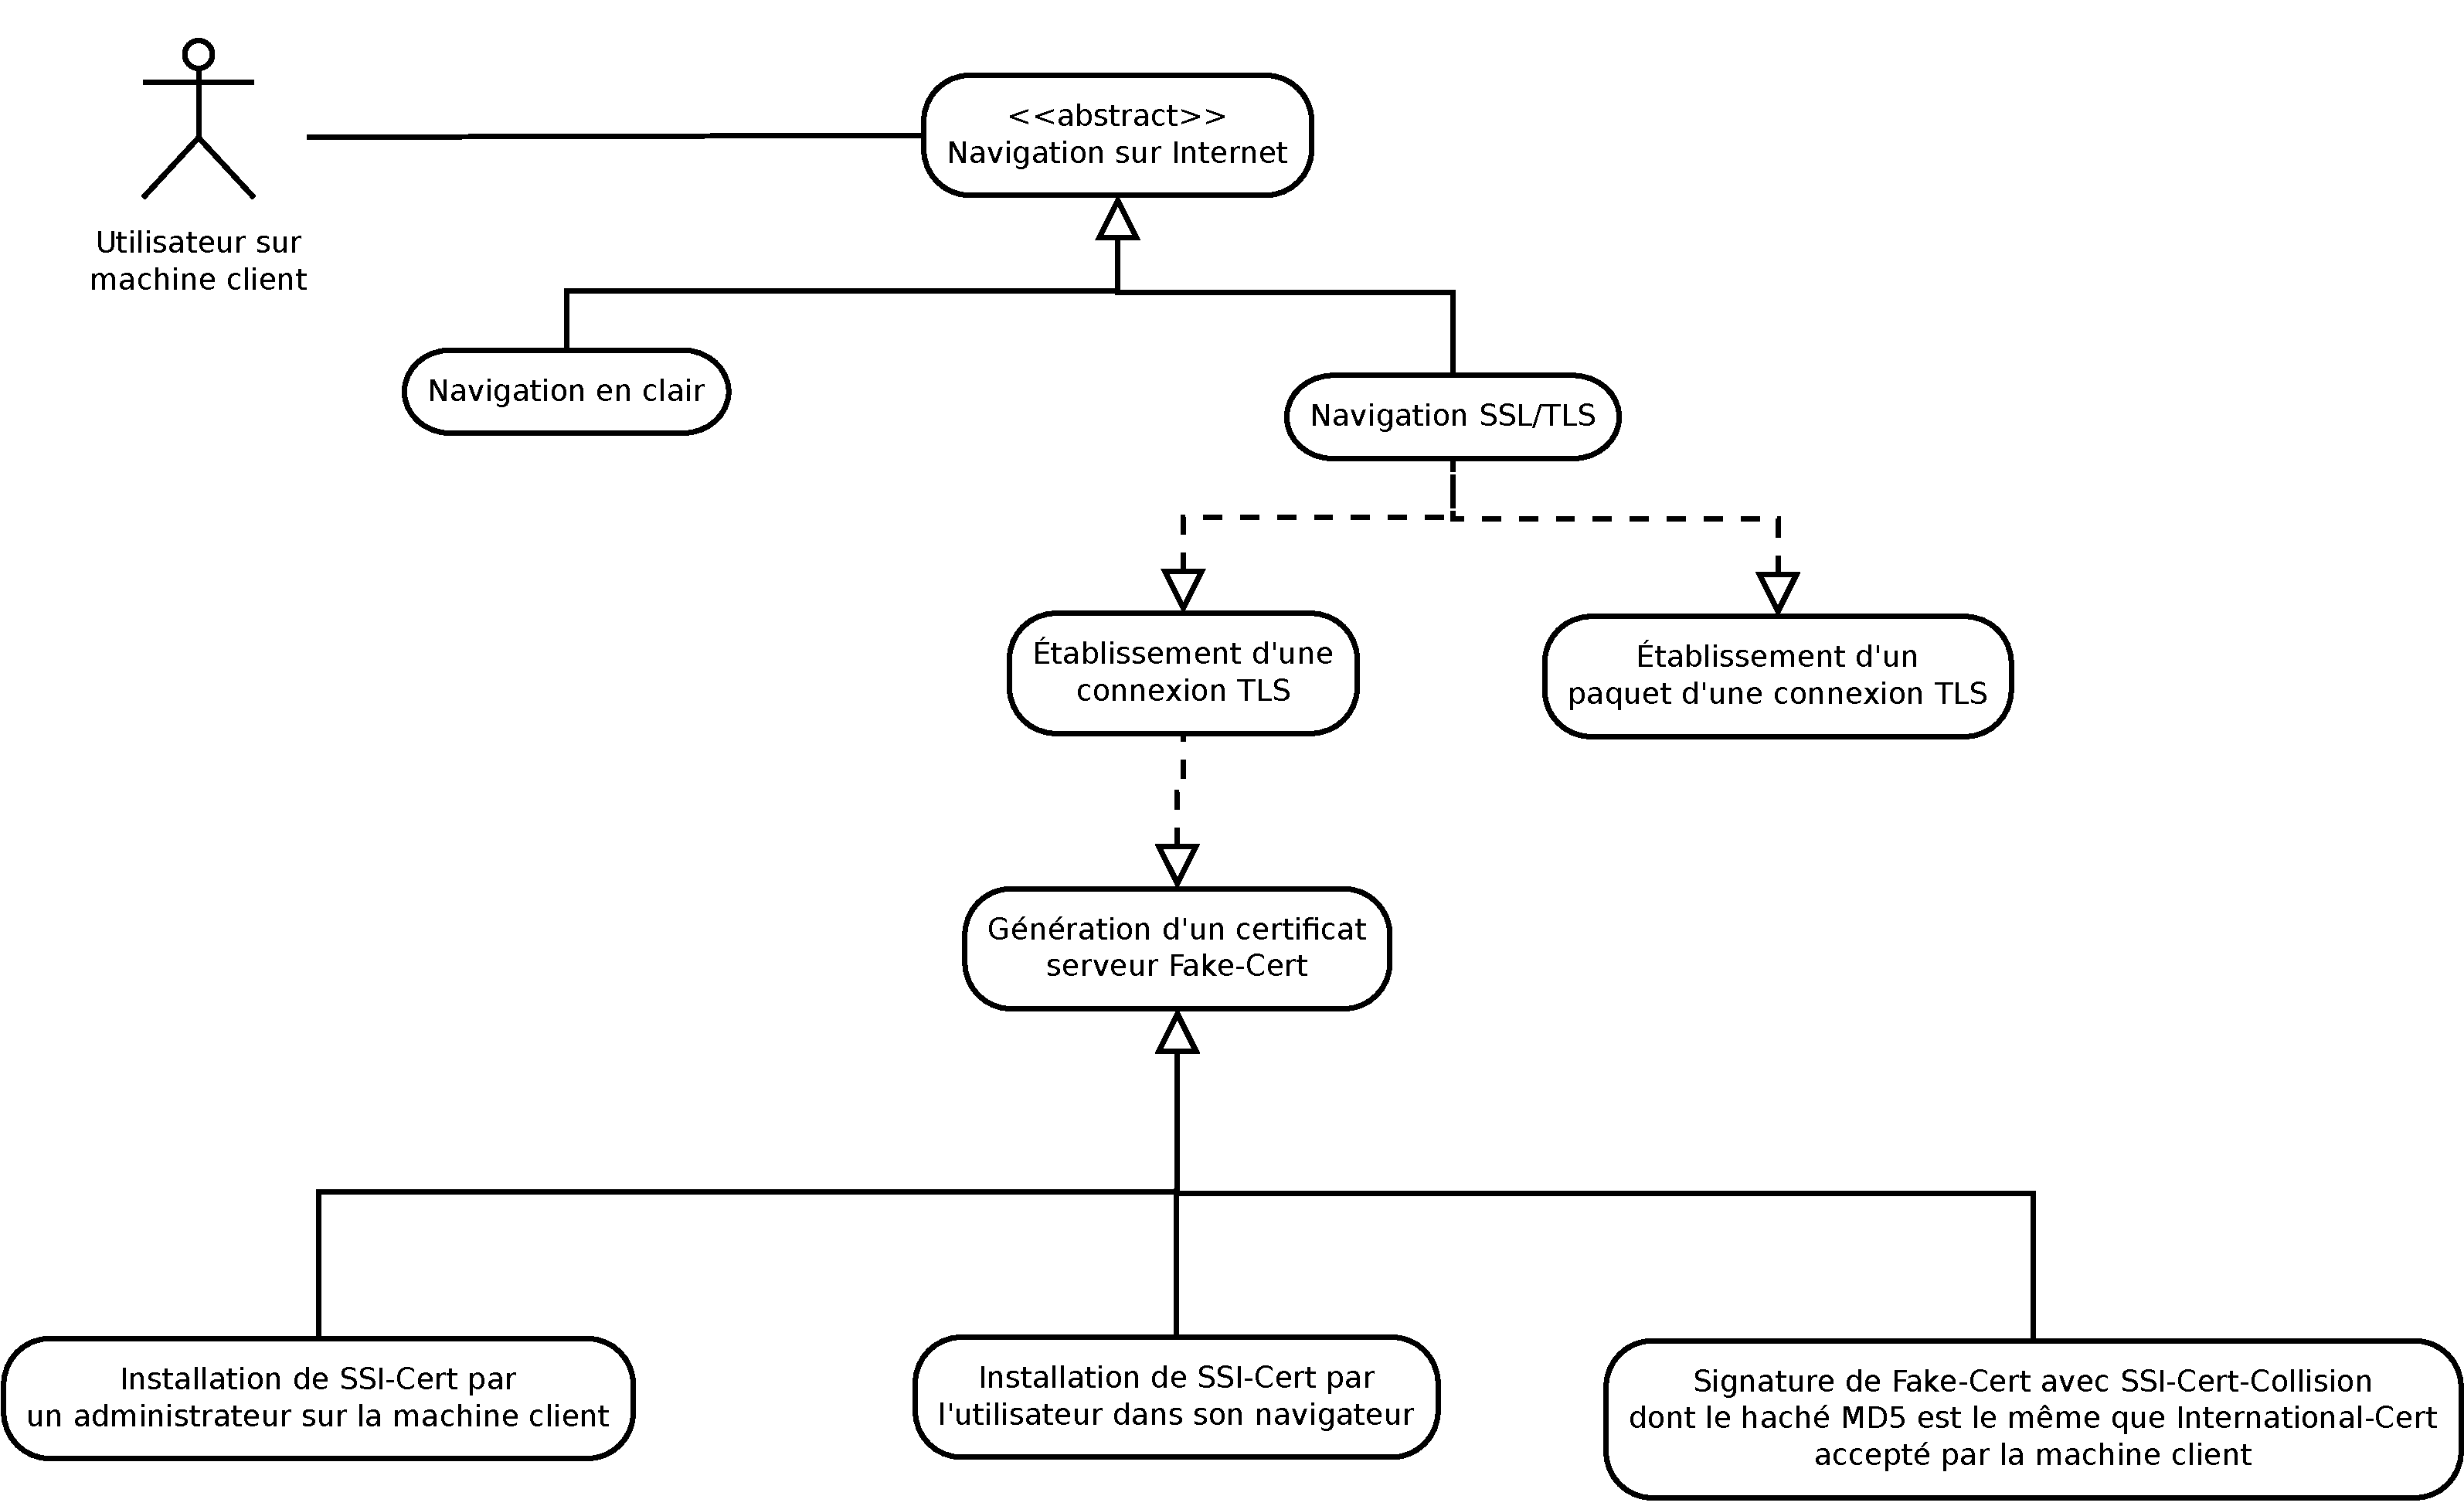
\includegraphics[width=\textwidth]{images/cas_utilisation.pdf}
\end{center}
\normalsize

\subsection{Schémas explicatifs}

\subsubsection{Phase de partage de certificats}

\begin{center}
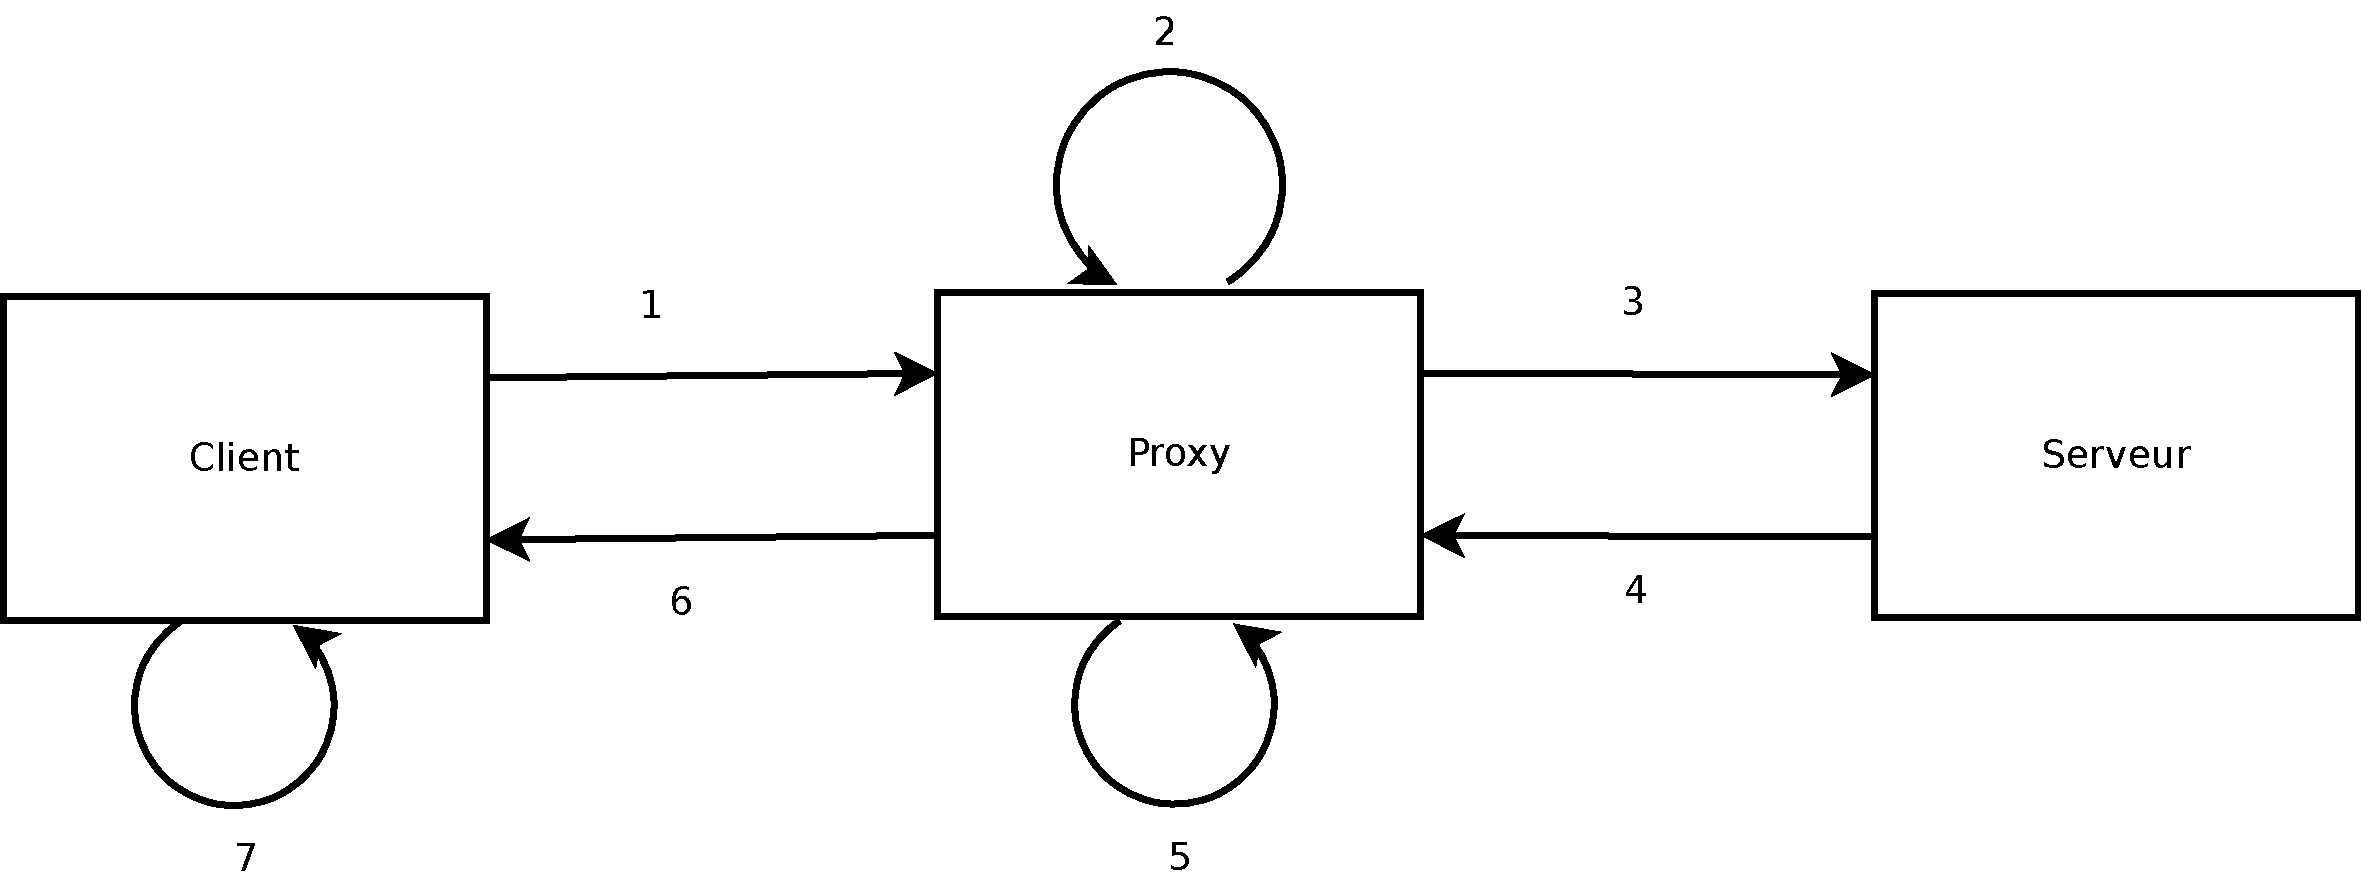
\includegraphics[width=\textwidth]{images/Certificats.pdf}
\end{center}

1. Le client envoie une requête au serveur pour négocier une connexion SSL/TLS.

2. Le proxy intercepte la requête.

3. Le proxy envoie sa propre requête de connexion au serveur demandé par le client.

4. Le serveur répond au proxy et envoie son certificat signé par une autorité.

5. Le proxy génère un faux certificat avec la clé publique du proxy et la signature de notre autorité.

6. Le proxy envoie le faux certificat au client.

7. Le client vérifie que le certificat est valide.\\

Une fois les certificats partagés, il faut maintenant échanger une clé de session pour avoir une connexion sécurisée.

\subsubsection{Phase d'échange des clés}

\begin{center}
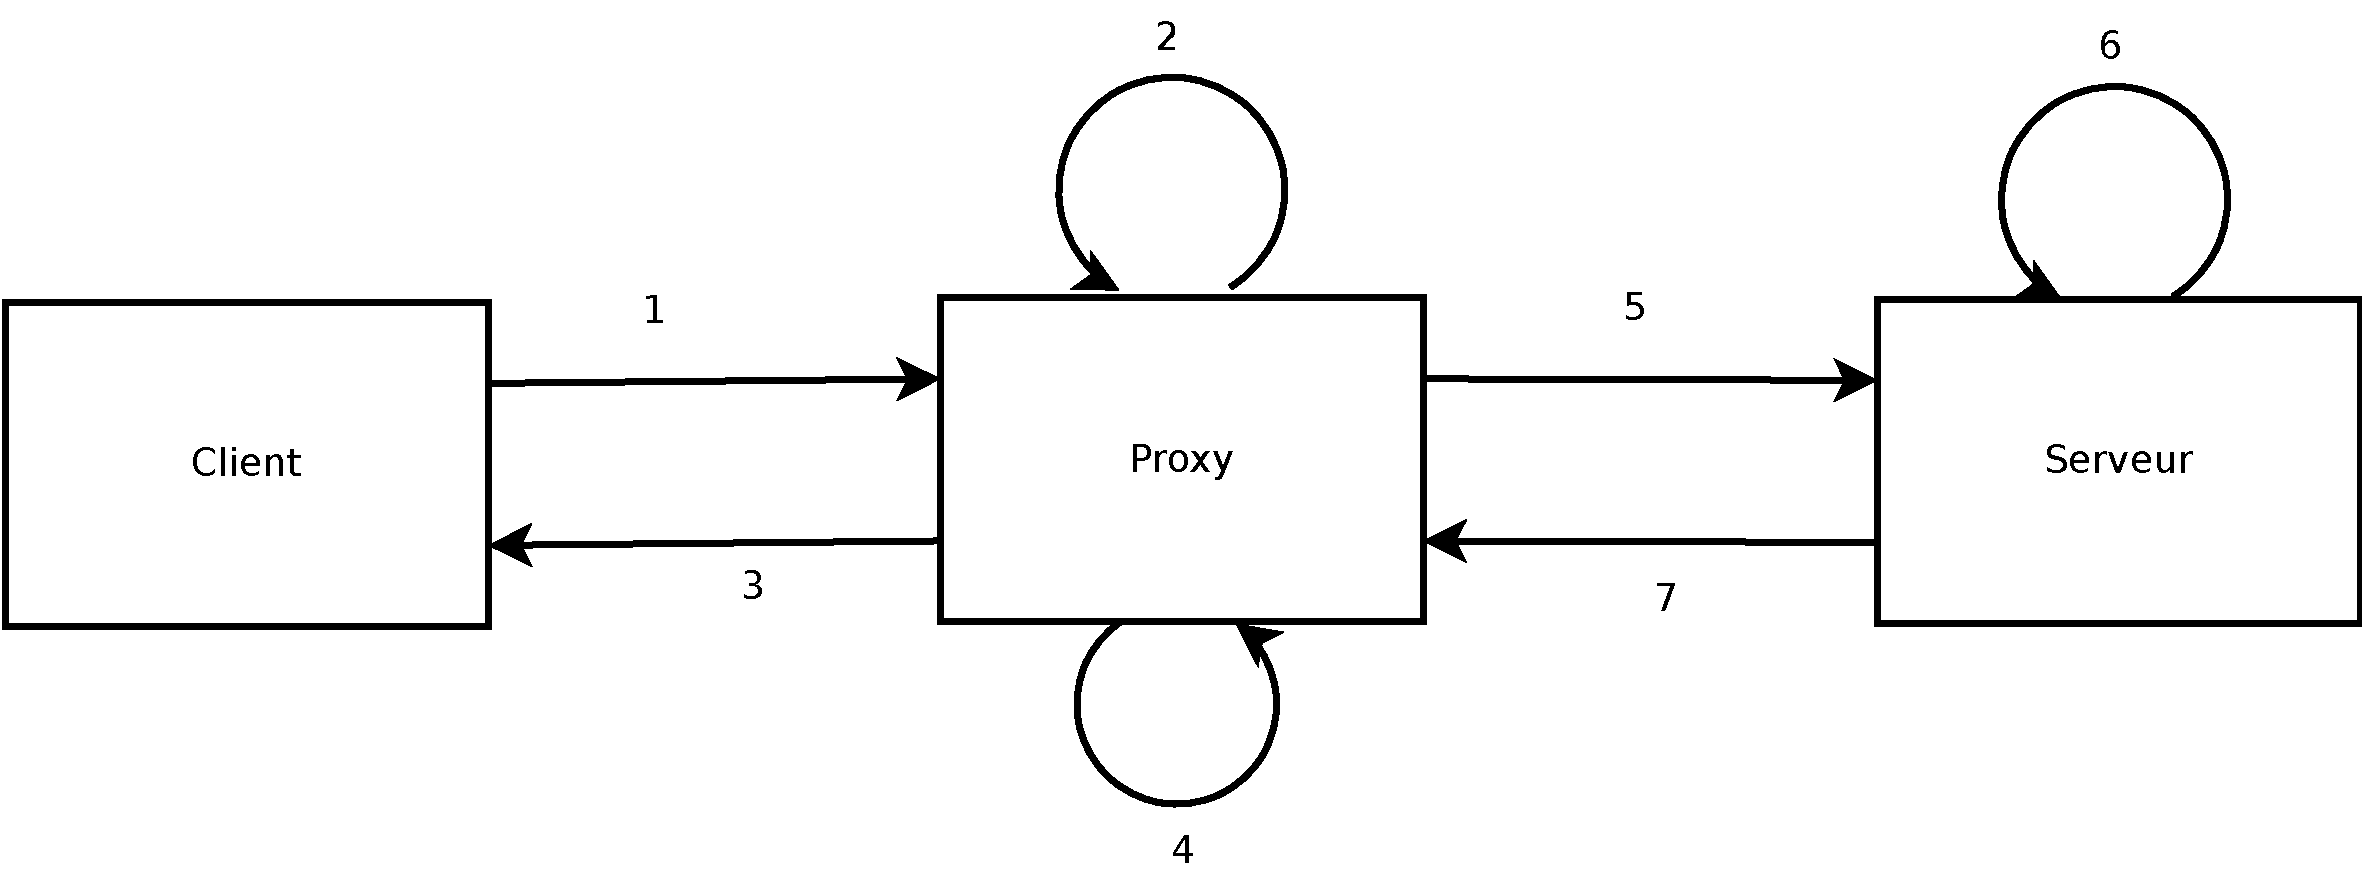
\includegraphics[width=\textwidth]{images/Cles.pdf}
\end{center}


1. Le client envoie une clé de session chiffrée avec la clé publique présente sur le certificat du proxy.

2. Le proxy déchiffre avec la clé privée associée.

3. Le proxy ouvre une connexion sécurisée avec le client avec la clé de session.

4. Le proxy chiffre une nouvelle clé de session avec la clé publique du serveur.

5. Le proxy envoie la clé chiffrée au serveur.

6. Le serveur déchiffre la clé de session.

7. Le serveur ouvre une connexion sécurisée avec le proxy en utilisant la clé de session.


\section{Cas d'utilisation}

\subsection{Configuration du proxy}

Installation et configuration du proxy pour que tout le trafic en provenance du client passe par le proxy.

\begin{tabular}{|>{\columncolor[gray]{.8}}m{4cm}|m{12cm}|}
   \hline
   Description & Mise en place du proxy \\
   \hline
   Pré-conditions & Implémentation du cas d'utilisation Transchiffrement\\
   \hline
   Évènement déclenchant & Début du projet \\
   \hline
   Condition d'arrêt & Proxy installé \\
   \hline
   Cas d'exception  &  \\
   \hline   
\end{tabular}

~\\

Description du flot d'évènements principal :

\begin{tabular}{|m{8cm}|m{8cm}|}
   \hline
   Acteur(s) & Système \\
   \hline
   1. Lancement de l'exécutable du proxy & \\
   \hline
\end{tabular}

\subsection{Installation de l'autorité}

Dans ce cas de figure, on prend l'exemple d'un administrateur système qui installe directement l'autorité sur les machines clientes.

\begin{tabular}{|>{\columncolor[gray]{.8}}m{4cm}|m{12cm}|}

   \hline
   Description & Première façon de faire : installer directement l'autorité dans le système\\
   \hline
   Pré-conditions &Autorité par défaut présente \\
   \hline
   Évènement déclenchant &  Mise en place de l'autorité\\
   \hline
   Condition d'arrêt & Autorité reconnue comme valide \\
   \hline
   Cas d'exception  & \\
   \hline   
\end{tabular}


~\\

Description du flot d'évènements principal :

\begin{tabular}{|m{8cm}|m{8cm}|}
   \hline
   Acteur(s) & Système \\
   \hline
   1. Installation de l'autorité directement dans le système du client. & \\
   \hline
\end{tabular}

\subsection{Acceptation de l'autorité}

Dans ce cas de figure, on veut forcer le client à accepter notre fausse autorité par une suite d'actions de paramétrage dans son navigateur.

\begin{tabular}{|>{\columncolor[gray]{.8}}m{4cm}|m{12cm}|}
   \hline
   Description & Deuxième façon de faire : faire accepter au client notre autorité.\\
   \hline
   Pré-conditions & Pas d'autorité présente\\
   \hline
   Évènement déclenchant & Première connexion au proxy par le client \\
   \hline
   Condition d'arrêt & Autorité reconnue comme valide \\
   \hline
   Cas d'exception  & L'autorité n'est pas acceptée par le client. \\
   \hline   
\end{tabular}

~\\

Description du flot d'évènements principal :

\begin{tabular}{|m{8cm}|m{8cm}|}
   \hline
  \rowcolor[gray]{.8} Acteur(s) & Système \\
   \hline
   1. Le client se connecte au proxy. & \\
   \hline
    & 2. Proposition de l'autorité au client. \\
   \hline
   3. Le client accepte et installe l'autorité. &  \\
   \hline
\end{tabular}


\subsection{Utilisation d'une fausse autorité forgée}

Si la deuxième partie du projet a donné un résultat, nous aurons donc réussi à forger un faux certificat d'autorité ayant le même haché MD5 que celui choisi.
Dans ce cas, nous utiliserons ce certificat.

\begin{tabular}{|>{\columncolor[gray]{.8}}m{4cm}|m{12cm}|}
   \hline
   Description & Utilisation d'une fausse autorité forgée \\
   \hline
   Pré-conditions & L'algorithme de recherche a renvoyé un certificat ayant le même haché MD5 que celui attendu.
 \\
   \hline
   Évènement déclenchant & L'algorithme de recherche a donné une réponse positive \\
   \hline
   Condition d'arrêt & L'autorité est reconnue comme valide \\
   \hline
   Cas d'exception  &  L'algorithme de recherche n'a pas donné le résultat voulu et nous n'utiliserons pas cette  façon de faire. \\
   \hline   
\end{tabular}

~\\

~\\

Description du flot d'évènements principal :

\begin{tabular}{|m{8cm}|m{8cm}|}
   \hline
  \rowcolor[gray]{.8} Acteur(s) & Système \\
   \hline
   1. Le client se connecte au proxy. & \\
   \hline
    & 2. Proposition de l'autorité au client. \\
   \hline
      3. Le client compare les hachés MD5 des deux autorités et l'accepte car ils sont égaux & \\
   \hline
    4. Le client installe l'autorité. &  \\
   \hline
\end{tabular}

\subsection{Génération de certificats}

Une fois l'autorité acceptée, à chaque demande de connexion HTTPS du client à un serveur, un faux certificat doit être généré à la volée.

\begin{tabular}{|>{\columncolor[gray]{.8}}m{4cm}|m{12cm}|}
   \hline
   Description & Génération d'un faux certificat pour le serveur \\
   \hline
   Pré-conditions & Le client ne s'est pas encore connecté à ce serveur \\
   \hline
   Évènement déclenchant & Le client tente de se connecter à un serveur \\
   \hline
   Condition d'arrêt &  Certificat généré et valide \\
   \hline
   Cas d'exception  &  Si le client s'est déjà connecté à ce serveur, on va le chercher dans une liste de certificats déjà générés auparavant.
\\
   \hline   
\end{tabular}

~\\

Description du flot d'évènements principal :

\begin{tabular}{|m{8cm}|m{8cm}|}
   \hline
  \rowcolor[gray]{.8} Acteur(s) & Système \\
   \hline
   1. Le client tente de se connecter à un serveur & \\
   \hline
    & 
2. Un faux certificat semblable en tout point au vrai est généré, seule la clé publique est remplacée par celle du proxy \\
   \hline
\end{tabular}

\subsection{Transchiffrement des paquets d'une connexion HTTPS}

Une fois le certificat généré, le client établit une connexion TLS/SSL et envoie sa requête au proxy de manière chiffrée, le proxy déchiffre, la garde dans les logs (éventuellement) puis rechiffre cette requête pour le serveur (avec une autre clé). Le but de ce processus est d'être transparent donc très rapide.
On a bien évidemment le même processus dans l'autre sens pour la réponse du serveur au client.

\begin{tabular}{|>{\columncolor[gray]{.8}}m{4cm}|m{12cm}|}
   \hline
   Description & Déchiffrement / Rechiffrement de la requête du client pour l'envoyer au serveur et de la réponse du serveur pour l'envoyer au client. \\
   \hline
   Pré-conditions & Certificat généré et deux connexions TLS/SSL ouvertes\\
   \hline
   Évènement déclenchant &  Envoi d'une requête du client\\
   \hline
   Condition d'arrêt & Message rédigé et transfert d’envoi terminé \\
   \hline
   Cas d'exception  & Renégociation TLS/SSL \\
   \hline   
\end{tabular}

~\\

Description du flot d'évènements principal :

\begin{tabular}{|m{8cm}|m{8cm}|}
   \hline
  \rowcolor[gray]{.8} Acteur(s) & Système \\
   \hline
   1. Envoi d'une requête chiffrée par le client & \\
   \hline
    &
2. Déchiffrement de la requête

3. Log de cette requête

4. Rechiffrement de la requête pour le serveur

5. Envoi de cette requête au serveur


8. Réception de la réponse chiffrée

9. Déchiffrement de la réponse

10. Log de la réponse
=======


>>>>>>> Stashed changes

<!DOCTYPE html>
<html>
  <head prefix="og: http://ogp.me/ns# fb: http://ogp.me/ns/fb# githubog: http://ogp.me/ns/fb/githubog#">
    <meta charset='utf-8'>
    <meta http-equiv="X-UA-Compatible" content="IE=edge">
        <title>Transchiffrement-doc/STB/STB.tex at master · nouafyve/Transchiffrement-doc</title>
    <link rel="search" type="application/opensearchdescription+xml" href="/opensearch.xml" title="GitHub" />
    <link rel="fluid-icon" href="https://github.com/fluidicon.png" title="GitHub" />
    <link rel="apple-touch-icon" sizes="57x57" href="/apple-touch-icon-114.png" />
    <link rel="apple-touch-icon" sizes="114x114" href="/apple-touch-icon-114.png" />
    <link rel="apple-touch-icon" sizes="72x72" href="/apple-touch-icon-144.png" />
    <link rel="apple-touch-icon" sizes="144x144" href="/apple-touch-icon-144.png" />
    <link rel="logo" type="image/svg" href="https://github-media-downloads.s3.amazonaws.com/github-logo.svg" />
    <meta property="og:image" content="https://github.global.ssl.fastly.net/images/modules/logos_page/Octocat.png">
    <meta name="hostname" content="github-fe116-cp1-prd.iad.github.net">
    <meta name="ruby" content="ruby 2.1.0p0-github-tcmalloc (60139581e1) [x86_64-linux]">
    <link rel="assets" href="https://github.global.ssl.fastly.net/">
    <link rel="conduit-xhr" href="https://ghconduit.com:25035/">
    <link rel="xhr-socket" href="/_sockets" />
    


    <meta name="msapplication-TileImage" content="/windows-tile.png" />
    <meta name="msapplication-TileColor" content="#ffffff" />
    <meta name="selected-link" value="repo_source" data-pjax-transient />
    <meta content="collector.githubapp.com" name="octolytics-host" /><meta content="collector-cdn.github.com" name="octolytics-script-host" /><meta content="github" name="octolytics-app-id" /><meta content="C134A230:2BC2:399BC6:52DD4D59" name="octolytics-dimension-request_id" /><meta content="6265276" name="octolytics-actor-id" /><meta content="wiss89" name="octolytics-actor-login" /><meta content="42367543e22ca7678eff2013b76483db6e2344d608f6031eae4e295771b35790" name="octolytics-actor-hash" />
    

    
    
    <link rel="icon" type="image/x-icon" href="/favicon.ico" />

    <meta content="authenticity_token" name="csrf-param" />
<meta content="8bWhJDp1LG2TSJnn2FQudVxqAEr3dm4Vh/q7NHwnBAI=" name="csrf-token" />

    <link href="https://github.global.ssl.fastly.net/assets/github-afd65da2802beafd8aee40df66e8b576092b2913.css" media="all" rel="stylesheet" type="text/css" />
    <link href="https://github.global.ssl.fastly.net/assets/github2-980ee38a688dc721bc8670970a05d3c5536d8daa.css" media="all" rel="stylesheet" type="text/css" />
    


      <script src="https://github.global.ssl.fastly.net/assets/frameworks-bf5987648bb83690ac0a5e955f74bbaf6ba44c4a.js" type="text/javascript"></script>
      <script async="async" defer="defer" src="https://github.global.ssl.fastly.net/assets/github-8f0f971134413bf7449fde4428a2d0683d647ca5.js" type="text/javascript"></script>
      
      <meta http-equiv="x-pjax-version" content="5fe7ec139c1bfc53297d312484aaf0e3">

        <link data-pjax-transient rel='permalink' href='/nouafyve/Transchiffrement-doc/blob/f75acb6fd60a418a8fca3c3085ac444933ae3978/STB/STB.tex'>
  <meta property="og:title" content="Transchiffrement-doc"/>
  <meta property="og:type" content="githubog:gitrepository"/>
  <meta property="og:url" content="https://github.com/nouafyve/Transchiffrement-doc"/>
  <meta property="og:image" content="https://github.global.ssl.fastly.net/images/gravatars/gravatar-user-420.png"/>
  <meta property="og:site_name" content="GitHub"/>
  <meta property="og:description" content="Contribute to Transchiffrement-doc development by creating an account on GitHub."/>

  <meta name="description" content="Contribute to Transchiffrement-doc development by creating an account on GitHub." />

  <meta content="2931323" name="octolytics-dimension-user_id" /><meta content="nouafyve" name="octolytics-dimension-user_login" /><meta content="14774016" name="octolytics-dimension-repository_id" /><meta content="nouafyve/Transchiffrement-doc" name="octolytics-dimension-repository_nwo" /><meta content="true" name="octolytics-dimension-repository_public" /><meta content="false" name="octolytics-dimension-repository_is_fork" /><meta content="14774016" name="octolytics-dimension-repository_network_root_id" /><meta content="nouafyve/Transchiffrement-doc" name="octolytics-dimension-repository_network_root_nwo" />
  <link href="https://github.com/nouafyve/Transchiffrement-doc/commits/master.atom" rel="alternate" title="Recent Commits to Transchiffrement-doc:master" type="application/atom+xml" />

  </head>


  <body class="logged_in  env-production linux vis-public page-blob">
    <div class="wrapper">
      
      
      
      


      <div class="header header-logged-in true">
  <div class="container clearfix">

    <a class="header-logo-invertocat" href="https://github.com/">
  <span class="mega-octicon octicon-mark-github"></span>
</a>

    
    <a href="/notifications" class="notification-indicator tooltipped downwards" data-gotokey="n" title="You have no unread notifications">
        <span class="mail-status all-read"></span>
</a>

      <div class="command-bar js-command-bar  in-repository">
          <form accept-charset="UTF-8" action="/search" class="command-bar-form" id="top_search_form" method="get">

<input type="text" data-hotkey=" s" name="q" id="js-command-bar-field" placeholder="Search or type a command" tabindex="1" autocapitalize="off"
    
    data-username="wiss89"
      data-repo="nouafyve/Transchiffrement-doc"
      data-branch="master"
      data-sha="694ba15b3e7f23492239459970d2651e876fe57e"
  >

    <input type="hidden" name="nwo" value="nouafyve/Transchiffrement-doc" />

    <div class="select-menu js-menu-container js-select-menu search-context-select-menu">
      <span class="minibutton select-menu-button js-menu-target">
        <span class="js-select-button">This repository</span>
      </span>

      <div class="select-menu-modal-holder js-menu-content js-navigation-container">
        <div class="select-menu-modal">

          <div class="select-menu-item js-navigation-item js-this-repository-navigation-item selected">
            <span class="select-menu-item-icon octicon octicon-check"></span>
            <input type="radio" class="js-search-this-repository" name="search_target" value="repository" checked="checked" />
            <div class="select-menu-item-text js-select-button-text">This repository</div>
          </div> <!-- /.select-menu-item -->

          <div class="select-menu-item js-navigation-item js-all-repositories-navigation-item">
            <span class="select-menu-item-icon octicon octicon-check"></span>
            <input type="radio" name="search_target" value="global" />
            <div class="select-menu-item-text js-select-button-text">All repositories</div>
          </div> <!-- /.select-menu-item -->

        </div>
      </div>
    </div>

  <span class="octicon help tooltipped downwards" title="Show command bar help">
    <span class="octicon octicon-question"></span>
  </span>


  <input type="hidden" name="ref" value="cmdform">

</form>
        <ul class="top-nav">
          <li class="explore"><a href="/explore">Explore</a></li>
            <li><a href="https://gist.github.com">Gist</a></li>
            <li><a href="/blog">Blog</a></li>
          <li><a href="https://help.github.com">Help</a></li>
        </ul>
      </div>

    


  <ul id="user-links">
    <li>
      <a href="/wiss89" class="name">
        <img height="20" src="https://0.gravatar.com/avatar/78e958e067d415bbe886de07175b3f5f?d=https%3A%2F%2Fidenticons.github.com%2Faf5937da73b82eadec24c423d74f7665.png&amp;r=x&amp;s=140" width="20" /> wiss89
      </a>
    </li>

      <li class="new-menu dropdown-toggle js-menu-container">
        <a href="#" class="js-menu-target tooltipped downwards" title="Create new…">
          <span class="octicon octicon-plus"></span>
          <span class="dropdown-arrow"></span>
        </a>

        <div class="js-menu-content">
        </div>
      </li>

      <li>
        <a href="/settings/profile" id="account_settings"
          class="tooltipped downwards"
          aria-label="Account settings (You have no verified emails)"
          title="Account settings (You have no verified emails)">
          <span class="octicon octicon-tools"></span>
        </a>
          <span class="settings-warning">!</span>
      </li>
      <li>
        <a class="tooltipped downwards" href="/logout" data-method="post" id="logout" title="Sign out" aria-label="Sign out">
          <span class="octicon octicon-log-out"></span>
        </a>
      </li>

  </ul>

<div class="js-new-dropdown-contents hidden">
  

<ul class="dropdown-menu">
  <li>
    <a href="/new"><span class="octicon octicon-repo-create"></span> New repository</a>
  </li>
  <li>
    <a href="/organizations/new"><span class="octicon octicon-organization"></span> New organization</a>
  </li>



    <li class="section-title">
      <span title="nouafyve/Transchiffrement-doc">This repository</span>
    </li>
      <li>
        <a href="/nouafyve/Transchiffrement-doc/issues/new"><span class="octicon octicon-issue-opened"></span> New issue</a>
      </li>
</ul>

</div>


    
  </div>
</div>

      

      

<div class="flash-global flash-warn">
<div class="container">

    <h2>
      You don't have any verified emails.  We recommend <a href="https://github.com/settings/emails">verifying</a> at least one email.
    </h2>
    <p>
      Email verification helps our support team help you in case you have any email issues or lose your password.
    </p>














</div>
</div>



          <div class="site" itemscope itemtype="http://schema.org/WebPage">
    
    <div class="pagehead repohead instapaper_ignore readability-menu">
      <div class="container">
        

<ul class="pagehead-actions">

    <li class="subscription">
      <form accept-charset="UTF-8" action="/notifications/subscribe" class="js-social-container" data-autosubmit="true" data-remote="true" method="post"><div style="margin:0;padding:0;display:inline"><input name="authenticity_token" type="hidden" value="8bWhJDp1LG2TSJnn2FQudVxqAEr3dm4Vh/q7NHwnBAI=" /></div>  <input id="repository_id" name="repository_id" type="hidden" value="14774016" />

    <div class="select-menu js-menu-container js-select-menu">
      <a class="social-count js-social-count" href="/nouafyve/Transchiffrement-doc/watchers">
        5
      </a>
      <span class="minibutton select-menu-button with-count js-menu-target" role="button" tabindex="0">
        <span class="js-select-button">
          <span class="octicon octicon-eye-unwatch"></span>
          Unwatch
        </span>
      </span>

      <div class="select-menu-modal-holder">
        <div class="select-menu-modal subscription-menu-modal js-menu-content">
          <div class="select-menu-header">
            <span class="select-menu-title">Notification status</span>
            <span class="octicon octicon-remove-close js-menu-close"></span>
          </div> <!-- /.select-menu-header -->

          <div class="select-menu-list js-navigation-container" role="menu">

            <div class="select-menu-item js-navigation-item " role="menuitem" tabindex="0">
              <span class="select-menu-item-icon octicon octicon-check"></span>
              <div class="select-menu-item-text">
                <input id="do_included" name="do" type="radio" value="included" />
                <h4>Not watching</h4>
                <span class="description">You only receive notifications for conversations in which you participate or are @mentioned.</span>
                <span class="js-select-button-text hidden-select-button-text">
                  <span class="octicon octicon-eye-watch"></span>
                  Watch
                </span>
              </div>
            </div> <!-- /.select-menu-item -->

            <div class="select-menu-item js-navigation-item selected" role="menuitem" tabindex="0">
              <span class="select-menu-item-icon octicon octicon octicon-check"></span>
              <div class="select-menu-item-text">
                <input checked="checked" id="do_subscribed" name="do" type="radio" value="subscribed" />
                <h4>Watching</h4>
                <span class="description">You receive notifications for all conversations in this repository.</span>
                <span class="js-select-button-text hidden-select-button-text">
                  <span class="octicon octicon-eye-unwatch"></span>
                  Unwatch
                </span>
              </div>
            </div> <!-- /.select-menu-item -->

            <div class="select-menu-item js-navigation-item " role="menuitem" tabindex="0">
              <span class="select-menu-item-icon octicon octicon-check"></span>
              <div class="select-menu-item-text">
                <input id="do_ignore" name="do" type="radio" value="ignore" />
                <h4>Ignoring</h4>
                <span class="description">You do not receive any notifications for conversations in this repository.</span>
                <span class="js-select-button-text hidden-select-button-text">
                  <span class="octicon octicon-mute"></span>
                  Stop ignoring
                </span>
              </div>
            </div> <!-- /.select-menu-item -->

          </div> <!-- /.select-menu-list -->

        </div> <!-- /.select-menu-modal -->
      </div> <!-- /.select-menu-modal-holder -->
    </div> <!-- /.select-menu -->

</form>
    </li>

  <li>
  

<<<<<<< Updated upstream
\subsection{Transfert des paquets HTTP}

Si le client tente de se connecter en HTTP à un serveur web, on ne fait que de transférer les paquets.

\begin{tabular}{|>{\columncolor[gray]{.8}}m{4cm}|m{12cm}|}
   \hline
   Description & Transfert des paquets en clair \\
   \hline
   Pré-conditions & Proxy configuré pour le HTTP\\
   \hline
   Évènement déclenchant &  Envoi d'une requête du client\\
   \hline
   Condition d'arrêt & Message rédigé et transfert d’envoi terminé \\
   \hline
   Cas d'exception  & \\
   \hline   
\end{tabular}
=======
  <div class="js-toggler-container js-social-container starring-container ">
    <a href="/nouafyve/Transchiffrement-doc/unstar"
      class="minibutton with-count js-toggler-target star-button starred upwards"
      title="Unstar this repository" data-remote="true" data-method="post" rel="nofollow">
      <span class="octicon octicon-star-delete"></span><span class="text">Unstar</span>
    </a>

    <a href="/nouafyve/Transchiffrement-doc/star"
      class="minibutton with-count js-toggler-target star-button unstarred upwards"
      title="Star this repository" data-remote="true" data-method="post" rel="nofollow">
      <span class="octicon octicon-star"></span><span class="text">Star</span>
    </a>

      <a class="social-count js-social-count" href="/nouafyve/Transchiffrement-doc/stargazers">
        0
      </a>
  </div>

  </li>


        <li>
          <a href="/nouafyve/Transchiffrement-doc/fork" class="minibutton with-count js-toggler-target fork-button lighter upwards" title="Fork this repo" rel="facebox nofollow">
            <span class="octicon octicon-git-branch-create"></span><span class="text">Fork</span>
          </a>
          <a href="/nouafyve/Transchiffrement-doc/network" class="social-count">0</a>
        </li>


</ul>

        <h1 itemscope itemtype="http://data-vocabulary.org/Breadcrumb" class="entry-title public">
          <span class="repo-label"><span>public</span></span>
          <span class="mega-octicon octicon-repo"></span>
          <span class="author">
            <a href="/nouafyve" class="url fn" itemprop="url" rel="author"><span itemprop="title">nouafyve</span></a>
          </span>
          <span class="repohead-name-divider">/</span>
          <strong><a href="/nouafyve/Transchiffrement-doc" class="js-current-repository js-repo-home-link">Transchiffrement-doc</a></strong>

          <span class="page-context-loader">
            <img alt="Octocat-spinner-32" height="16" src="https://github.global.ssl.fastly.net/images/spinners/octocat-spinner-32.gif" width="16" />
          </span>

        </h1>
      </div><!-- /.container -->
    </div><!-- /.repohead -->

    <div class="container">
      

      <div class="repository-with-sidebar repo-container  ">

        <div class="repository-sidebar">
            

<div class="sunken-menu vertical-right repo-nav js-repo-nav js-repository-container-pjax js-octicon-loaders">
  <div class="sunken-menu-contents">
    <ul class="sunken-menu-group">
      <li class="tooltipped leftwards" title="Code">
        <a href="/nouafyve/Transchiffrement-doc" aria-label="Code" class="selected js-selected-navigation-item sunken-menu-item" data-gotokey="c" data-pjax="true" data-selected-links="repo_source repo_downloads repo_commits repo_tags repo_branches /nouafyve/Transchiffrement-doc">
          <span class="octicon octicon-code"></span> <span class="full-word">Code</span>
          <img alt="Octocat-spinner-32" class="mini-loader" height="16" src="https://github.global.ssl.fastly.net/images/spinners/octocat-spinner-32.gif" width="16" />
</a>      </li>

        <li class="tooltipped leftwards" title="Issues">
          <a href="/nouafyve/Transchiffrement-doc/issues" aria-label="Issues" class="js-selected-navigation-item sunken-menu-item js-disable-pjax" data-gotokey="i" data-selected-links="repo_issues /nouafyve/Transchiffrement-doc/issues">
            <span class="octicon octicon-issue-opened"></span> <span class="full-word">Issues</span>
            <span class='counter'>0</span>
            <img alt="Octocat-spinner-32" class="mini-loader" height="16" src="https://github.global.ssl.fastly.net/images/spinners/octocat-spinner-32.gif" width="16" />
</a>        </li>

      <li class="tooltipped leftwards" title="Pull Requests">
        <a href="/nouafyve/Transchiffrement-doc/pulls" aria-label="Pull Requests" class="js-selected-navigation-item sunken-menu-item js-disable-pjax" data-gotokey="p" data-selected-links="repo_pulls /nouafyve/Transchiffrement-doc/pulls">
            <span class="octicon octicon-git-pull-request"></span> <span class="full-word">Pull Requests</span>
            <span class='counter'>0</span>
            <img alt="Octocat-spinner-32" class="mini-loader" height="16" src="https://github.global.ssl.fastly.net/images/spinners/octocat-spinner-32.gif" width="16" />
</a>      </li>


        <li class="tooltipped leftwards" title="Wiki">
          <a href="/nouafyve/Transchiffrement-doc/wiki" aria-label="Wiki" class="js-selected-navigation-item sunken-menu-item" data-pjax="true" data-selected-links="repo_wiki /nouafyve/Transchiffrement-doc/wiki">
            <span class="octicon octicon-book"></span> <span class="full-word">Wiki</span>
            <img alt="Octocat-spinner-32" class="mini-loader" height="16" src="https://github.global.ssl.fastly.net/images/spinners/octocat-spinner-32.gif" width="16" />
</a>        </li>
    </ul>
    <div class="sunken-menu-separator"></div>
    <ul class="sunken-menu-group">

      <li class="tooltipped leftwards" title="Pulse">
        <a href="/nouafyve/Transchiffrement-doc/pulse" aria-label="Pulse" class="js-selected-navigation-item sunken-menu-item" data-pjax="true" data-selected-links="pulse /nouafyve/Transchiffrement-doc/pulse">
          <span class="octicon octicon-pulse"></span> <span class="full-word">Pulse</span>
          <img alt="Octocat-spinner-32" class="mini-loader" height="16" src="https://github.global.ssl.fastly.net/images/spinners/octocat-spinner-32.gif" width="16" />
</a>      </li>

      <li class="tooltipped leftwards" title="Graphs">
        <a href="/nouafyve/Transchiffrement-doc/graphs" aria-label="Graphs" class="js-selected-navigation-item sunken-menu-item" data-pjax="true" data-selected-links="repo_graphs repo_contributors /nouafyve/Transchiffrement-doc/graphs">
          <span class="octicon octicon-graph"></span> <span class="full-word">Graphs</span>
          <img alt="Octocat-spinner-32" class="mini-loader" height="16" src="https://github.global.ssl.fastly.net/images/spinners/octocat-spinner-32.gif" width="16" />
</a>      </li>

      <li class="tooltipped leftwards" title="Network">
        <a href="/nouafyve/Transchiffrement-doc/network" aria-label="Network" class="js-selected-navigation-item sunken-menu-item js-disable-pjax" data-selected-links="repo_network /nouafyve/Transchiffrement-doc/network">
          <span class="octicon octicon-git-branch"></span> <span class="full-word">Network</span>
          <img alt="Octocat-spinner-32" class="mini-loader" height="16" src="https://github.global.ssl.fastly.net/images/spinners/octocat-spinner-32.gif" width="16" />
</a>      </li>
    </ul>


  </div>
</div>

            <div class="only-with-full-nav">
              

  

<div class="clone-url open"
  data-protocol-type="http"
  data-url="/users/set_protocol?protocol_selector=http&amp;protocol_type=push">
  <h3><strong>HTTPS</strong> clone URL</h3>
  <div class="clone-url-box">
    <input type="text" class="clone js-url-field"
           value="https://github.com/nouafyve/Transchiffrement-doc.git" readonly="readonly">

    <span class="js-zeroclipboard url-box-clippy minibutton zeroclipboard-button" data-clipboard-text="https://github.com/nouafyve/Transchiffrement-doc.git" data-copied-hint="copied!" title="copy to clipboard"><span class="octicon octicon-clippy"></span></span>
  </div>
</div>
>>>>>>> Stashed changes

  

<div class="clone-url "
  data-protocol-type="ssh"
  data-url="/users/set_protocol?protocol_selector=ssh&amp;protocol_type=push">
  <h3><strong>SSH</strong> clone URL</h3>
  <div class="clone-url-box">
    <input type="text" class="clone js-url-field"
           value="git@github.com:nouafyve/Transchiffrement-doc.git" readonly="readonly">

<<<<<<< Updated upstream
Description du flot d'évènements principal :

\begin{tabular}{|m{8cm}|m{8cm}|}
   \hline
  \rowcolor[gray]{.8} Acteur(s) & Système \\
   \hline
   1. Envoi d'une requête en clair par le client & \\
   \hline
& 2. Transfert de la requête au serveur  \\
& 3. Réception de la réponse du serveur  \\
   \hline
  
4. Envoi de la réponse au client  &  \\
   \hline
\end{tabular}

\section{Etude}

Notre étude porte sur la recherche de seconde pré-image du MD5.\\
Nous devons comprendre le fonctionnement de MD5 et utiliser la faiblesse de cet algorithme.\\
Nous allons développer un algorithme de recherche pour générer un certificat d'autorité ayant le même haché qu'un existant choisi.\\
Nous savons que le champ qui permet le plus de modifications est celui de la clé publique du certificat.\\
Grâce à une étude réalisée en 2008, nous savons quels champs nous pouvons modifier pour que le haché MD5 soit le plus proche de l'original.\\
C'est donc sur les bits du modulo de la clé publique que nous allons opérer la majeure partie des changements.\\
Pour que ce certificat d'autorité soit considéré comme valide, il faut que le haché de ce certificat soit le même que celui que nous voulons imiter.\\
Si nous arrivons à générer un certificat d'autorité remplissant cette condition, nous pourrons l'inclure dans le proxy de transchiffrement.\\
Nous serons donc capables de signer les certificats générés à la volée quand un utilisateur veut y avoir accès.\\
Grâce à ces faux-certificats, nous pourrons alors voir tout ce qui transite sans que l'utilisateur s'en aperçoive.\\
Nous allons donc livrer un rapport d'étude pour expliquer notre démarche pour la création de l'algorithme.\\
=======
    <span class="js-zeroclipboard url-box-clippy minibutton zeroclipboard-button" data-clipboard-text="git@github.com:nouafyve/Transchiffrement-doc.git" data-copied-hint="copied!" title="copy to clipboard"><span class="octicon octicon-clippy"></span></span>
  </div>
</div>

  

<div class="clone-url "
  data-protocol-type="subversion"
  data-url="/users/set_protocol?protocol_selector=subversion&amp;protocol_type=push">
  <h3><strong>Subversion</strong> checkout URL</h3>
  <div class="clone-url-box">
    <input type="text" class="clone js-url-field"
           value="https://github.com/nouafyve/Transchiffrement-doc" readonly="readonly">

    <span class="js-zeroclipboard url-box-clippy minibutton zeroclipboard-button" data-clipboard-text="https://github.com/nouafyve/Transchiffrement-doc" data-copied-hint="copied!" title="copy to clipboard"><span class="octicon octicon-clippy"></span></span>
  </div>
</div>


<p class="clone-options">You can clone with
      <a href="#" class="js-clone-selector" data-protocol="http">HTTPS</a>,
      <a href="#" class="js-clone-selector" data-protocol="ssh">SSH</a>,
      or <a href="#" class="js-clone-selector" data-protocol="subversion">Subversion</a>.
  <span class="octicon help tooltipped upwards" title="Get help on which URL is right for you.">
    <a href="https://help.github.com/articles/which-remote-url-should-i-use">
    <span class="octicon octicon-question"></span>
    </a>
  </span>
</p>


\section{Performances}
Pour que notre proxy soit considéré comme "transparent", nous devons remplir des contraintes de temps d'exécution du transchiffrement.
On s'autorise donc une seconde de marge pour toute page générée très rapidement et jusqu'à 200\% du temps pour une page contenant un volume conséquent de données.

              <a href="/nouafyve/Transchiffrement-doc/archive/master.zip"
                 class="minibutton sidebar-button"
                 title="Download this repository as a zip file"
                 rel="nofollow">
                <span class="octicon octicon-cloud-download"></span>
                Download ZIP
              </a>
            </div>
        </div><!-- /.repository-sidebar -->

        <div id="js-repo-pjax-container" class="repository-content context-loader-container" data-pjax-container>
          


<!-- blob contrib key: blob_contributors:v21:0d20a80301abfefebf267882e927963a -->

<p title="This is a placeholder element" class="js-history-link-replace hidden"></p>

<a href="/nouafyve/Transchiffrement-doc/find/master" data-pjax data-hotkey="t" class="js-show-file-finder" style="display:none">Show File Finder</a>

<div class="file-navigation">
  
>>>>>>> Stashed changes

<div class="select-menu js-menu-container js-select-menu" >
  <span class="minibutton select-menu-button js-menu-target" data-hotkey="w"
    data-master-branch="master"
    data-ref="master"
    role="button" aria-label="Switch branches or tags" tabindex="0">
    <span class="octicon octicon-git-branch"></span>
    <i>branch:</i>
    <span class="js-select-button">master</span>
  </span>

  <div class="select-menu-modal-holder js-menu-content js-navigation-container" data-pjax>

    <div class="select-menu-modal">
      <div class="select-menu-header">
        <span class="select-menu-title">Switch branches/tags</span>
        <span class="octicon octicon-remove-close js-menu-close"></span>
      </div> <!-- /.select-menu-header -->

      <div class="select-menu-filters">
        <div class="select-menu-text-filter">
          <input type="text" aria-label="Find or create a branch…" id="context-commitish-filter-field" class="js-filterable-field js-navigation-enable" placeholder="Find or create a branch…">
        </div>
        <div class="select-menu-tabs">
          <ul>
            <li class="select-menu-tab">
              <a href="#" data-tab-filter="branches" class="js-select-menu-tab">Branches</a>
            </li>
            <li class="select-menu-tab">
              <a href="#" data-tab-filter="tags" class="js-select-menu-tab">Tags</a>
            </li>
          </ul>
        </div><!-- /.select-menu-tabs -->
      </div><!-- /.select-menu-filters -->

      <div class="select-menu-list select-menu-tab-bucket js-select-menu-tab-bucket" data-tab-filter="branches">

        <div data-filterable-for="context-commitish-filter-field" data-filterable-type="substring">


            <div class="select-menu-item js-navigation-item selected">
              <span class="select-menu-item-icon octicon octicon-check"></span>
              <a href="/nouafyve/Transchiffrement-doc/blob/master/STB/STB.tex"
                 data-name="master"
                 data-skip-pjax="true"
                 rel="nofollow"
                 class="js-navigation-open select-menu-item-text js-select-button-text css-truncate-target"
                 title="master">master</a>
            </div> <!-- /.select-menu-item -->
        </div>

          <form accept-charset="UTF-8" action="/nouafyve/Transchiffrement-doc/branches" class="js-create-branch select-menu-item select-menu-new-item-form js-navigation-item js-new-item-form" method="post"><div style="margin:0;padding:0;display:inline"><input name="authenticity_token" type="hidden" value="8bWhJDp1LG2TSJnn2FQudVxqAEr3dm4Vh/q7NHwnBAI=" /></div>
            <span class="octicon octicon-git-branch-create select-menu-item-icon"></span>
            <div class="select-menu-item-text">
              <h4>Create branch: <span class="js-new-item-name"></span></h4>
              <span class="description">from ‘master’</span>
            </div>
            <input type="hidden" name="name" id="name" class="js-new-item-value">
            <input type="hidden" name="branch" id="branch" value="master" />
            <input type="hidden" name="path" id="path" value="STB/STB.tex" />
          </form> <!-- /.select-menu-item -->

      </div> <!-- /.select-menu-list -->

      <div class="select-menu-list select-menu-tab-bucket js-select-menu-tab-bucket" data-tab-filter="tags">
        <div data-filterable-for="context-commitish-filter-field" data-filterable-type="substring">


        </div>

        <div class="select-menu-no-results">Nothing to show</div>
      </div> <!-- /.select-menu-list -->

    </div> <!-- /.select-menu-modal -->
  </div> <!-- /.select-menu-modal-holder -->
</div> <!-- /.select-menu -->

  <div class="breadcrumb">
    <span class='repo-root js-repo-root'><span itemscope="" itemtype="http://data-vocabulary.org/Breadcrumb"><a href="/nouafyve/Transchiffrement-doc" data-branch="master" data-direction="back" data-pjax="true" itemscope="url"><span itemprop="title">Transchiffrement-doc</span></a></span></span><span class="separator"> / </span><span itemscope="" itemtype="http://data-vocabulary.org/Breadcrumb"><a href="/nouafyve/Transchiffrement-doc/tree/master/STB" data-branch="master" data-direction="back" data-pjax="true" itemscope="url"><span itemprop="title">STB</span></a></span><span class="separator"> / </span><strong class="final-path">STB.tex</strong> <span class="js-zeroclipboard minibutton zeroclipboard-button" data-clipboard-text="STB/STB.tex" data-copied-hint="copied!" title="copy to clipboard"><span class="octicon octicon-clippy"></span></span>
  </div>
</div>



  <div class="commit file-history-tease">
    <img class="main-avatar" height="24" src="https://2.gravatar.com/avatar/abc200c4909022b3f80420bd4392fa00?d=https%3A%2F%2Fidenticons.github.com%2F4571650eff31af4bd7950d61322a27c3.png&amp;r=x&amp;s=140" width="24" />
    <span class="author"><a href="/Pyrow" rel="author">Pyrow</a></span>
    <time class="js-relative-date" datetime="2014-01-20T08:10:37-08:00" title="2014-01-20 08:10:37">January 20, 2014</time>
    <div class="commit-title">
        <a href="/nouafyve/Transchiffrement-doc/commit/6f5f4c9e4e7f22552350a13ec0e07d45db4f125f" class="message" data-pjax="true" title="Ajout STB finie">Ajout STB finie</a>
    </div>

    <div class="participation">
      <p class="quickstat"><a href="#blob_contributors_box" rel="facebox"><strong>1</strong> contributor</a></p>
      
    </div>
    <div id="blob_contributors_box" style="display:none">
      <h2 class="facebox-header">Users who have contributed to this file</h2>
      <ul class="facebox-user-list">
          <li class="facebox-user-list-item">
            <img height="24" src="https://2.gravatar.com/avatar/abc200c4909022b3f80420bd4392fa00?d=https%3A%2F%2Fidenticons.github.com%2F4571650eff31af4bd7950d61322a27c3.png&amp;r=x&amp;s=140" width="24" />
            <a href="/Pyrow">Pyrow</a>
          </li>
      </ul>
    </div>
  </div>

<div id="files" class="bubble">
  <div class="file">
    <div class="meta">
      <div class="info">
        <span class="icon"><b class="octicon octicon-file-text"></b></span>
        <span class="mode" title="File Mode">file</span>
          <span>513 lines (394 sloc)</span>
        <span>17.332 kb</span>
      </div>
      <div class="actions">
        <div class="button-group">
                <a class="minibutton"
                   href="/nouafyve/Transchiffrement-doc/edit/master/STB/STB.tex"
                   data-method="post" rel="nofollow" data-hotkey="e">Edit</a>
          <a href="/nouafyve/Transchiffrement-doc/raw/master/STB/STB.tex" class="button minibutton " id="raw-url">Raw</a>
            <a href="/nouafyve/Transchiffrement-doc/blame/master/STB/STB.tex" class="button minibutton ">Blame</a>
          <a href="/nouafyve/Transchiffrement-doc/commits/master/STB/STB.tex" class="button minibutton " rel="nofollow">History</a>
        </div><!-- /.button-group -->
          <a class="minibutton danger empty-icon tooltipped downwards"
             href="/nouafyve/Transchiffrement-doc/delete/master/STB/STB.tex"
             title=""
             data-method="post" data-test-id="delete-blob-file" rel="nofollow">
          Delete
        </a>
      </div><!-- /.actions -->

    </div>
        <div class="blob-wrapper data type-tex js-blob-data">
        <table class="file-code file-diff">
          <tr class="file-code-line">
            <td class="blob-line-nums">
              <span id="L1" rel="#L1">1</span>
<span id="L2" rel="#L2">2</span>
<span id="L3" rel="#L3">3</span>
<span id="L4" rel="#L4">4</span>
<span id="L5" rel="#L5">5</span>
<span id="L6" rel="#L6">6</span>
<span id="L7" rel="#L7">7</span>
<span id="L8" rel="#L8">8</span>
<span id="L9" rel="#L9">9</span>
<span id="L10" rel="#L10">10</span>
<span id="L11" rel="#L11">11</span>
<span id="L12" rel="#L12">12</span>
<span id="L13" rel="#L13">13</span>
<span id="L14" rel="#L14">14</span>
<span id="L15" rel="#L15">15</span>
<span id="L16" rel="#L16">16</span>
<span id="L17" rel="#L17">17</span>
<span id="L18" rel="#L18">18</span>
<span id="L19" rel="#L19">19</span>
<span id="L20" rel="#L20">20</span>
<span id="L21" rel="#L21">21</span>
<span id="L22" rel="#L22">22</span>
<span id="L23" rel="#L23">23</span>
<span id="L24" rel="#L24">24</span>
<span id="L25" rel="#L25">25</span>
<span id="L26" rel="#L26">26</span>
<span id="L27" rel="#L27">27</span>
<span id="L28" rel="#L28">28</span>
<span id="L29" rel="#L29">29</span>
<span id="L30" rel="#L30">30</span>
<span id="L31" rel="#L31">31</span>
<span id="L32" rel="#L32">32</span>
<span id="L33" rel="#L33">33</span>
<span id="L34" rel="#L34">34</span>
<span id="L35" rel="#L35">35</span>
<span id="L36" rel="#L36">36</span>
<span id="L37" rel="#L37">37</span>
<span id="L38" rel="#L38">38</span>
<span id="L39" rel="#L39">39</span>
<span id="L40" rel="#L40">40</span>
<span id="L41" rel="#L41">41</span>
<span id="L42" rel="#L42">42</span>
<span id="L43" rel="#L43">43</span>
<span id="L44" rel="#L44">44</span>
<span id="L45" rel="#L45">45</span>
<span id="L46" rel="#L46">46</span>
<span id="L47" rel="#L47">47</span>
<span id="L48" rel="#L48">48</span>
<span id="L49" rel="#L49">49</span>
<span id="L50" rel="#L50">50</span>
<span id="L51" rel="#L51">51</span>
<span id="L52" rel="#L52">52</span>
<span id="L53" rel="#L53">53</span>
<span id="L54" rel="#L54">54</span>
<span id="L55" rel="#L55">55</span>
<span id="L56" rel="#L56">56</span>
<span id="L57" rel="#L57">57</span>
<span id="L58" rel="#L58">58</span>
<span id="L59" rel="#L59">59</span>
<span id="L60" rel="#L60">60</span>
<span id="L61" rel="#L61">61</span>
<span id="L62" rel="#L62">62</span>
<span id="L63" rel="#L63">63</span>
<span id="L64" rel="#L64">64</span>
<span id="L65" rel="#L65">65</span>
<span id="L66" rel="#L66">66</span>
<span id="L67" rel="#L67">67</span>
<span id="L68" rel="#L68">68</span>
<span id="L69" rel="#L69">69</span>
<span id="L70" rel="#L70">70</span>
<span id="L71" rel="#L71">71</span>
<span id="L72" rel="#L72">72</span>
<span id="L73" rel="#L73">73</span>
<span id="L74" rel="#L74">74</span>
<span id="L75" rel="#L75">75</span>
<span id="L76" rel="#L76">76</span>
<span id="L77" rel="#L77">77</span>
<span id="L78" rel="#L78">78</span>
<span id="L79" rel="#L79">79</span>
<span id="L80" rel="#L80">80</span>
<span id="L81" rel="#L81">81</span>
<span id="L82" rel="#L82">82</span>
<span id="L83" rel="#L83">83</span>
<span id="L84" rel="#L84">84</span>
<span id="L85" rel="#L85">85</span>
<span id="L86" rel="#L86">86</span>
<span id="L87" rel="#L87">87</span>
<span id="L88" rel="#L88">88</span>
<span id="L89" rel="#L89">89</span>
<span id="L90" rel="#L90">90</span>
<span id="L91" rel="#L91">91</span>
<span id="L92" rel="#L92">92</span>
<span id="L93" rel="#L93">93</span>
<span id="L94" rel="#L94">94</span>
<span id="L95" rel="#L95">95</span>
<span id="L96" rel="#L96">96</span>
<span id="L97" rel="#L97">97</span>
<span id="L98" rel="#L98">98</span>
<span id="L99" rel="#L99">99</span>
<span id="L100" rel="#L100">100</span>
<span id="L101" rel="#L101">101</span>
<span id="L102" rel="#L102">102</span>
<span id="L103" rel="#L103">103</span>
<span id="L104" rel="#L104">104</span>
<span id="L105" rel="#L105">105</span>
<span id="L106" rel="#L106">106</span>
<span id="L107" rel="#L107">107</span>
<span id="L108" rel="#L108">108</span>
<span id="L109" rel="#L109">109</span>
<span id="L110" rel="#L110">110</span>
<span id="L111" rel="#L111">111</span>
<span id="L112" rel="#L112">112</span>
<span id="L113" rel="#L113">113</span>
<span id="L114" rel="#L114">114</span>
<span id="L115" rel="#L115">115</span>
<span id="L116" rel="#L116">116</span>
<span id="L117" rel="#L117">117</span>
<span id="L118" rel="#L118">118</span>
<span id="L119" rel="#L119">119</span>
<span id="L120" rel="#L120">120</span>
<span id="L121" rel="#L121">121</span>
<span id="L122" rel="#L122">122</span>
<span id="L123" rel="#L123">123</span>
<span id="L124" rel="#L124">124</span>
<span id="L125" rel="#L125">125</span>
<span id="L126" rel="#L126">126</span>
<span id="L127" rel="#L127">127</span>
<span id="L128" rel="#L128">128</span>
<span id="L129" rel="#L129">129</span>
<span id="L130" rel="#L130">130</span>
<span id="L131" rel="#L131">131</span>
<span id="L132" rel="#L132">132</span>
<span id="L133" rel="#L133">133</span>
<span id="L134" rel="#L134">134</span>
<span id="L135" rel="#L135">135</span>
<span id="L136" rel="#L136">136</span>
<span id="L137" rel="#L137">137</span>
<span id="L138" rel="#L138">138</span>
<span id="L139" rel="#L139">139</span>
<span id="L140" rel="#L140">140</span>
<span id="L141" rel="#L141">141</span>
<span id="L142" rel="#L142">142</span>
<span id="L143" rel="#L143">143</span>
<span id="L144" rel="#L144">144</span>
<span id="L145" rel="#L145">145</span>
<span id="L146" rel="#L146">146</span>
<span id="L147" rel="#L147">147</span>
<span id="L148" rel="#L148">148</span>
<span id="L149" rel="#L149">149</span>
<span id="L150" rel="#L150">150</span>
<span id="L151" rel="#L151">151</span>
<span id="L152" rel="#L152">152</span>
<span id="L153" rel="#L153">153</span>
<span id="L154" rel="#L154">154</span>
<span id="L155" rel="#L155">155</span>
<span id="L156" rel="#L156">156</span>
<span id="L157" rel="#L157">157</span>
<span id="L158" rel="#L158">158</span>
<span id="L159" rel="#L159">159</span>
<span id="L160" rel="#L160">160</span>
<span id="L161" rel="#L161">161</span>
<span id="L162" rel="#L162">162</span>
<span id="L163" rel="#L163">163</span>
<span id="L164" rel="#L164">164</span>
<span id="L165" rel="#L165">165</span>
<span id="L166" rel="#L166">166</span>
<span id="L167" rel="#L167">167</span>
<span id="L168" rel="#L168">168</span>
<span id="L169" rel="#L169">169</span>
<span id="L170" rel="#L170">170</span>
<span id="L171" rel="#L171">171</span>
<span id="L172" rel="#L172">172</span>
<span id="L173" rel="#L173">173</span>
<span id="L174" rel="#L174">174</span>
<span id="L175" rel="#L175">175</span>
<span id="L176" rel="#L176">176</span>
<span id="L177" rel="#L177">177</span>
<span id="L178" rel="#L178">178</span>
<span id="L179" rel="#L179">179</span>
<span id="L180" rel="#L180">180</span>
<span id="L181" rel="#L181">181</span>
<span id="L182" rel="#L182">182</span>
<span id="L183" rel="#L183">183</span>
<span id="L184" rel="#L184">184</span>
<span id="L185" rel="#L185">185</span>
<span id="L186" rel="#L186">186</span>
<span id="L187" rel="#L187">187</span>
<span id="L188" rel="#L188">188</span>
<span id="L189" rel="#L189">189</span>
<span id="L190" rel="#L190">190</span>
<span id="L191" rel="#L191">191</span>
<span id="L192" rel="#L192">192</span>
<span id="L193" rel="#L193">193</span>
<span id="L194" rel="#L194">194</span>
<span id="L195" rel="#L195">195</span>
<span id="L196" rel="#L196">196</span>
<span id="L197" rel="#L197">197</span>
<span id="L198" rel="#L198">198</span>
<span id="L199" rel="#L199">199</span>
<span id="L200" rel="#L200">200</span>
<span id="L201" rel="#L201">201</span>
<span id="L202" rel="#L202">202</span>
<span id="L203" rel="#L203">203</span>
<span id="L204" rel="#L204">204</span>
<span id="L205" rel="#L205">205</span>
<span id="L206" rel="#L206">206</span>
<span id="L207" rel="#L207">207</span>
<span id="L208" rel="#L208">208</span>
<span id="L209" rel="#L209">209</span>
<span id="L210" rel="#L210">210</span>
<span id="L211" rel="#L211">211</span>
<span id="L212" rel="#L212">212</span>
<span id="L213" rel="#L213">213</span>
<span id="L214" rel="#L214">214</span>
<span id="L215" rel="#L215">215</span>
<span id="L216" rel="#L216">216</span>
<span id="L217" rel="#L217">217</span>
<span id="L218" rel="#L218">218</span>
<span id="L219" rel="#L219">219</span>
<span id="L220" rel="#L220">220</span>
<span id="L221" rel="#L221">221</span>
<span id="L222" rel="#L222">222</span>
<span id="L223" rel="#L223">223</span>
<span id="L224" rel="#L224">224</span>
<span id="L225" rel="#L225">225</span>
<span id="L226" rel="#L226">226</span>
<span id="L227" rel="#L227">227</span>
<span id="L228" rel="#L228">228</span>
<span id="L229" rel="#L229">229</span>
<span id="L230" rel="#L230">230</span>
<span id="L231" rel="#L231">231</span>
<span id="L232" rel="#L232">232</span>
<span id="L233" rel="#L233">233</span>
<span id="L234" rel="#L234">234</span>
<span id="L235" rel="#L235">235</span>
<span id="L236" rel="#L236">236</span>
<span id="L237" rel="#L237">237</span>
<span id="L238" rel="#L238">238</span>
<span id="L239" rel="#L239">239</span>
<span id="L240" rel="#L240">240</span>
<span id="L241" rel="#L241">241</span>
<span id="L242" rel="#L242">242</span>
<span id="L243" rel="#L243">243</span>
<span id="L244" rel="#L244">244</span>
<span id="L245" rel="#L245">245</span>
<span id="L246" rel="#L246">246</span>
<span id="L247" rel="#L247">247</span>
<span id="L248" rel="#L248">248</span>
<span id="L249" rel="#L249">249</span>
<span id="L250" rel="#L250">250</span>
<span id="L251" rel="#L251">251</span>
<span id="L252" rel="#L252">252</span>
<span id="L253" rel="#L253">253</span>
<span id="L254" rel="#L254">254</span>
<span id="L255" rel="#L255">255</span>
<span id="L256" rel="#L256">256</span>
<span id="L257" rel="#L257">257</span>
<span id="L258" rel="#L258">258</span>
<span id="L259" rel="#L259">259</span>
<span id="L260" rel="#L260">260</span>
<span id="L261" rel="#L261">261</span>
<span id="L262" rel="#L262">262</span>
<span id="L263" rel="#L263">263</span>
<span id="L264" rel="#L264">264</span>
<span id="L265" rel="#L265">265</span>
<span id="L266" rel="#L266">266</span>
<span id="L267" rel="#L267">267</span>
<span id="L268" rel="#L268">268</span>
<span id="L269" rel="#L269">269</span>
<span id="L270" rel="#L270">270</span>
<span id="L271" rel="#L271">271</span>
<span id="L272" rel="#L272">272</span>
<span id="L273" rel="#L273">273</span>
<span id="L274" rel="#L274">274</span>
<span id="L275" rel="#L275">275</span>
<span id="L276" rel="#L276">276</span>
<span id="L277" rel="#L277">277</span>
<span id="L278" rel="#L278">278</span>
<span id="L279" rel="#L279">279</span>
<span id="L280" rel="#L280">280</span>
<span id="L281" rel="#L281">281</span>
<span id="L282" rel="#L282">282</span>
<span id="L283" rel="#L283">283</span>
<span id="L284" rel="#L284">284</span>
<span id="L285" rel="#L285">285</span>
<span id="L286" rel="#L286">286</span>
<span id="L287" rel="#L287">287</span>
<span id="L288" rel="#L288">288</span>
<span id="L289" rel="#L289">289</span>
<span id="L290" rel="#L290">290</span>
<span id="L291" rel="#L291">291</span>
<span id="L292" rel="#L292">292</span>
<span id="L293" rel="#L293">293</span>
<span id="L294" rel="#L294">294</span>
<span id="L295" rel="#L295">295</span>
<span id="L296" rel="#L296">296</span>
<span id="L297" rel="#L297">297</span>
<span id="L298" rel="#L298">298</span>
<span id="L299" rel="#L299">299</span>
<span id="L300" rel="#L300">300</span>
<span id="L301" rel="#L301">301</span>
<span id="L302" rel="#L302">302</span>
<span id="L303" rel="#L303">303</span>
<span id="L304" rel="#L304">304</span>
<span id="L305" rel="#L305">305</span>
<span id="L306" rel="#L306">306</span>
<span id="L307" rel="#L307">307</span>
<span id="L308" rel="#L308">308</span>
<span id="L309" rel="#L309">309</span>
<span id="L310" rel="#L310">310</span>
<span id="L311" rel="#L311">311</span>
<span id="L312" rel="#L312">312</span>
<span id="L313" rel="#L313">313</span>
<span id="L314" rel="#L314">314</span>
<span id="L315" rel="#L315">315</span>
<span id="L316" rel="#L316">316</span>
<span id="L317" rel="#L317">317</span>
<span id="L318" rel="#L318">318</span>
<span id="L319" rel="#L319">319</span>
<span id="L320" rel="#L320">320</span>
<span id="L321" rel="#L321">321</span>
<span id="L322" rel="#L322">322</span>
<span id="L323" rel="#L323">323</span>
<span id="L324" rel="#L324">324</span>
<span id="L325" rel="#L325">325</span>
<span id="L326" rel="#L326">326</span>
<span id="L327" rel="#L327">327</span>
<span id="L328" rel="#L328">328</span>
<span id="L329" rel="#L329">329</span>
<span id="L330" rel="#L330">330</span>
<span id="L331" rel="#L331">331</span>
<span id="L332" rel="#L332">332</span>
<span id="L333" rel="#L333">333</span>
<span id="L334" rel="#L334">334</span>
<span id="L335" rel="#L335">335</span>
<span id="L336" rel="#L336">336</span>
<span id="L337" rel="#L337">337</span>
<span id="L338" rel="#L338">338</span>
<span id="L339" rel="#L339">339</span>
<span id="L340" rel="#L340">340</span>
<span id="L341" rel="#L341">341</span>
<span id="L342" rel="#L342">342</span>
<span id="L343" rel="#L343">343</span>
<span id="L344" rel="#L344">344</span>
<span id="L345" rel="#L345">345</span>
<span id="L346" rel="#L346">346</span>
<span id="L347" rel="#L347">347</span>
<span id="L348" rel="#L348">348</span>
<span id="L349" rel="#L349">349</span>
<span id="L350" rel="#L350">350</span>
<span id="L351" rel="#L351">351</span>
<span id="L352" rel="#L352">352</span>
<span id="L353" rel="#L353">353</span>
<span id="L354" rel="#L354">354</span>
<span id="L355" rel="#L355">355</span>
<span id="L356" rel="#L356">356</span>
<span id="L357" rel="#L357">357</span>
<span id="L358" rel="#L358">358</span>
<span id="L359" rel="#L359">359</span>
<span id="L360" rel="#L360">360</span>
<span id="L361" rel="#L361">361</span>
<span id="L362" rel="#L362">362</span>
<span id="L363" rel="#L363">363</span>
<span id="L364" rel="#L364">364</span>
<span id="L365" rel="#L365">365</span>
<span id="L366" rel="#L366">366</span>
<span id="L367" rel="#L367">367</span>
<span id="L368" rel="#L368">368</span>
<span id="L369" rel="#L369">369</span>
<span id="L370" rel="#L370">370</span>
<span id="L371" rel="#L371">371</span>
<span id="L372" rel="#L372">372</span>
<span id="L373" rel="#L373">373</span>
<span id="L374" rel="#L374">374</span>
<span id="L375" rel="#L375">375</span>
<span id="L376" rel="#L376">376</span>
<span id="L377" rel="#L377">377</span>
<span id="L378" rel="#L378">378</span>
<span id="L379" rel="#L379">379</span>
<span id="L380" rel="#L380">380</span>
<span id="L381" rel="#L381">381</span>
<span id="L382" rel="#L382">382</span>
<span id="L383" rel="#L383">383</span>
<span id="L384" rel="#L384">384</span>
<span id="L385" rel="#L385">385</span>
<span id="L386" rel="#L386">386</span>
<span id="L387" rel="#L387">387</span>
<span id="L388" rel="#L388">388</span>
<span id="L389" rel="#L389">389</span>
<span id="L390" rel="#L390">390</span>
<span id="L391" rel="#L391">391</span>
<span id="L392" rel="#L392">392</span>
<span id="L393" rel="#L393">393</span>
<span id="L394" rel="#L394">394</span>
<span id="L395" rel="#L395">395</span>
<span id="L396" rel="#L396">396</span>
<span id="L397" rel="#L397">397</span>
<span id="L398" rel="#L398">398</span>
<span id="L399" rel="#L399">399</span>
<span id="L400" rel="#L400">400</span>
<span id="L401" rel="#L401">401</span>
<span id="L402" rel="#L402">402</span>
<span id="L403" rel="#L403">403</span>
<span id="L404" rel="#L404">404</span>
<span id="L405" rel="#L405">405</span>
<span id="L406" rel="#L406">406</span>
<span id="L407" rel="#L407">407</span>
<span id="L408" rel="#L408">408</span>
<span id="L409" rel="#L409">409</span>
<span id="L410" rel="#L410">410</span>
<span id="L411" rel="#L411">411</span>
<span id="L412" rel="#L412">412</span>
<span id="L413" rel="#L413">413</span>
<span id="L414" rel="#L414">414</span>
<span id="L415" rel="#L415">415</span>
<span id="L416" rel="#L416">416</span>
<span id="L417" rel="#L417">417</span>
<span id="L418" rel="#L418">418</span>
<span id="L419" rel="#L419">419</span>
<span id="L420" rel="#L420">420</span>
<span id="L421" rel="#L421">421</span>
<span id="L422" rel="#L422">422</span>
<span id="L423" rel="#L423">423</span>
<span id="L424" rel="#L424">424</span>
<span id="L425" rel="#L425">425</span>
<span id="L426" rel="#L426">426</span>
<span id="L427" rel="#L427">427</span>
<span id="L428" rel="#L428">428</span>
<span id="L429" rel="#L429">429</span>
<span id="L430" rel="#L430">430</span>
<span id="L431" rel="#L431">431</span>
<span id="L432" rel="#L432">432</span>
<span id="L433" rel="#L433">433</span>
<span id="L434" rel="#L434">434</span>
<span id="L435" rel="#L435">435</span>
<span id="L436" rel="#L436">436</span>
<span id="L437" rel="#L437">437</span>
<span id="L438" rel="#L438">438</span>
<span id="L439" rel="#L439">439</span>
<span id="L440" rel="#L440">440</span>
<span id="L441" rel="#L441">441</span>
<span id="L442" rel="#L442">442</span>
<span id="L443" rel="#L443">443</span>
<span id="L444" rel="#L444">444</span>
<span id="L445" rel="#L445">445</span>
<span id="L446" rel="#L446">446</span>
<span id="L447" rel="#L447">447</span>
<span id="L448" rel="#L448">448</span>
<span id="L449" rel="#L449">449</span>
<span id="L450" rel="#L450">450</span>
<span id="L451" rel="#L451">451</span>
<span id="L452" rel="#L452">452</span>
<span id="L453" rel="#L453">453</span>
<span id="L454" rel="#L454">454</span>
<span id="L455" rel="#L455">455</span>
<span id="L456" rel="#L456">456</span>
<span id="L457" rel="#L457">457</span>
<span id="L458" rel="#L458">458</span>
<span id="L459" rel="#L459">459</span>
<span id="L460" rel="#L460">460</span>
<span id="L461" rel="#L461">461</span>
<span id="L462" rel="#L462">462</span>
<span id="L463" rel="#L463">463</span>
<span id="L464" rel="#L464">464</span>
<span id="L465" rel="#L465">465</span>
<span id="L466" rel="#L466">466</span>
<span id="L467" rel="#L467">467</span>
<span id="L468" rel="#L468">468</span>
<span id="L469" rel="#L469">469</span>
<span id="L470" rel="#L470">470</span>
<span id="L471" rel="#L471">471</span>
<span id="L472" rel="#L472">472</span>
<span id="L473" rel="#L473">473</span>
<span id="L474" rel="#L474">474</span>
<span id="L475" rel="#L475">475</span>
<span id="L476" rel="#L476">476</span>
<span id="L477" rel="#L477">477</span>
<span id="L478" rel="#L478">478</span>
<span id="L479" rel="#L479">479</span>
<span id="L480" rel="#L480">480</span>
<span id="L481" rel="#L481">481</span>
<span id="L482" rel="#L482">482</span>
<span id="L483" rel="#L483">483</span>
<span id="L484" rel="#L484">484</span>
<span id="L485" rel="#L485">485</span>
<span id="L486" rel="#L486">486</span>
<span id="L487" rel="#L487">487</span>
<span id="L488" rel="#L488">488</span>
<span id="L489" rel="#L489">489</span>
<span id="L490" rel="#L490">490</span>
<span id="L491" rel="#L491">491</span>
<span id="L492" rel="#L492">492</span>
<span id="L493" rel="#L493">493</span>
<span id="L494" rel="#L494">494</span>
<span id="L495" rel="#L495">495</span>
<span id="L496" rel="#L496">496</span>
<span id="L497" rel="#L497">497</span>
<span id="L498" rel="#L498">498</span>
<span id="L499" rel="#L499">499</span>
<span id="L500" rel="#L500">500</span>
<span id="L501" rel="#L501">501</span>
<span id="L502" rel="#L502">502</span>
<span id="L503" rel="#L503">503</span>
<span id="L504" rel="#L504">504</span>
<span id="L505" rel="#L505">505</span>
<span id="L506" rel="#L506">506</span>
<span id="L507" rel="#L507">507</span>
<span id="L508" rel="#L508">508</span>
<span id="L509" rel="#L509">509</span>
<span id="L510" rel="#L510">510</span>
<span id="L511" rel="#L511">511</span>
<span id="L512" rel="#L512">512</span>
<span id="L513" rel="#L513">513</span>

            </td>
            <td class="blob-line-code">
                    <div class="code-body highlight"><pre><div class='line' id='LC1'><span class="k">\documentclass</span><span class="na">[a4paper,11pt,french]</span><span class="nb">{</span>article<span class="nb">}</span></div><div class='line' id='LC2'><span class="k">\usepackage</span><span class="na">[utf8]</span><span class="nb">{</span>inputenc<span class="nb">}</span></div><div class='line' id='LC3'><br/></div><div class='line' id='LC4'><span class="k">\usepackage</span><span class="na">[T1]</span><span class="nb">{</span>fontenc<span class="nb">}</span></div><div class='line' id='LC5'><span class="k">\usepackage</span><span class="na">[francais]</span><span class="nb">{</span>babel<span class="nb">}</span> </div><div class='line' id='LC6'><span class="k">\usepackage</span><span class="na">[top=2cm, bottom=2cm, left=2cm, right=2cm, includeheadfoot]</span><span class="nb">{</span>geometry<span class="nb">}</span> <span class="c">%pour les marges</span></div><div class='line' id='LC7'><span class="k">\usepackage</span><span class="nb">{</span>lmodern<span class="nb">}</span></div><div class='line' id='LC8'><span class="k">\usepackage</span><span class="nb">{</span>pict2e<span class="nb">}</span></div><div class='line' id='LC9'><span class="k">\usepackage</span><span class="nb">{</span>fancyhdr<span class="nb">}</span> <span class="c">% Required for custom headers</span></div><div class='line' id='LC10'><span class="k">\usepackage</span><span class="nb">{</span>lastpage<span class="nb">}</span> <span class="c">% Required to determine the last page for the footer</span></div><div class='line' id='LC11'><span class="k">\usepackage</span><span class="nb">{</span>extramarks<span class="nb">}</span> <span class="c">% Required for headers and footers</span></div><div class='line' id='LC12'><span class="k">\usepackage</span><span class="nb">{</span>graphicx<span class="nb">}</span> <span class="c">% Required to insert images</span></div><div class='line' id='LC13'><span class="k">\usepackage</span><span class="nb">{</span>tabularx, longtable<span class="nb">}</span></div><div class='line' id='LC14'><span class="k">\usepackage</span><span class="nb">{</span>color, colortbl<span class="nb">}</span></div><div class='line' id='LC15'><span class="k">\usepackage</span><span class="nb">{</span>lscape<span class="nb">}</span></div><div class='line' id='LC16'><span class="c">%\usepackage[hidelinks]{hyperref}</span></div><div class='line' id='LC17'><span class="k">\usepackage</span><span class="nb">{</span>longtable<span class="nb">}</span></div><div class='line' id='LC18'><span class="k">\usepackage</span><span class="nb">{</span>multirow<span class="nb">}</span></div><div class='line' id='LC19'><span class="k">\usepackage</span><span class="nb">{</span>rotating<span class="nb">}</span></div><div class='line' id='LC20'><span class="c">%\usepackage{pgfgantt}</span></div><div class='line' id='LC21'><span class="c">%\usepackage{pgfcalendar}</span></div><div class='line' id='LC22'><span class="c">%\usepackage{ifthen}</span></div><div class='line' id='LC23'><span class="k">\usepackage</span><span class="nb">{</span>gensymb<span class="nb">}</span></div><div class='line' id='LC24'><br/></div><div class='line' id='LC25'><span class="k">\linespread</span><span class="nb">{</span>1.1<span class="nb">}</span> <span class="c">% Line spacing</span></div><div class='line' id='LC26'><br/></div><div class='line' id='LC27'><span class="c">% Set up the header and footer</span></div><div class='line' id='LC28'><span class="k">\pagestyle</span><span class="nb">{</span>fancy<span class="nb">}</span></div><div class='line' id='LC29'><span class="k">\lhead</span><span class="nb">{</span><span class="k">\textbf</span><span class="nb">{</span><span class="k">\hmwkClass</span> -- <span class="k">\hmwkSubject</span> <span class="k">\\</span> <span class="k">\hmwkTitle</span> <span class="k">\\</span> <span class="k">\hmwkDocName</span><span class="nb">}}</span> <span class="c">% Top left header</span></div><div class='line' id='LC30'><span class="k">\rhead</span><span class="nb">{</span><span class="k">\includegraphics</span><span class="na">[width=10em]</span><span class="nb">{</span>logo<span class="nb">_</span>univ.png<span class="nb">}}</span></div><div class='line' id='LC31'><span class="k">\lfoot</span><span class="nb">{</span><span class="k">\lastxmark</span><span class="nb">}</span> <span class="c">% Bottom left footer</span></div><div class='line' id='LC32'><span class="k">\cfoot</span><span class="nb">{}</span> <span class="c">% Bottom center footer</span></div><div class='line' id='LC33'><span class="k">\rfoot</span><span class="nb">{</span>Page<span class="k">\ \thepage\ </span>/ <span class="k">\pageref</span><span class="nb">{</span>LastPage<span class="nb">}}</span> <span class="c">% Bottom right footer</span></div><div class='line' id='LC34'><span class="k">\renewcommand\headrulewidth</span><span class="nb">{</span>0.4pt<span class="nb">}</span> <span class="c">% Size of the header rule</span></div><div class='line' id='LC35'><span class="k">\renewcommand\footrulewidth</span><span class="nb">{</span>0.4pt<span class="nb">}</span> <span class="c">% Size of the footer rule</span></div><div class='line' id='LC36'><br/></div><div class='line' id='LC37'><span class="k">\setlength</span><span class="nb">{</span><span class="k">\headheight</span><span class="nb">}{</span>40pt<span class="nb">}</span></div><div class='line' id='LC38'><br/></div><div class='line' id='LC39'><span class="k">\newcommand</span><span class="nb">{</span><span class="k">\hmwkTitle</span><span class="nb">}{</span>Transchiffrement<span class="nb">}</span> <span class="c">% Assignment title</span></div><div class='line' id='LC40'><span class="k">\newcommand</span><span class="nb">{</span><span class="k">\hmwkClass</span><span class="nb">}{</span>Master 2 SSI <span class="nb">}</span> <span class="c">% Course/class</span></div><div class='line' id='LC41'><span class="k">\newcommand</span><span class="nb">{</span><span class="k">\hmwkAuthorName</span><span class="nb">}{</span>Julien Bourdon<span class="nb">}</span> <span class="c">% Your name</span></div><div class='line' id='LC42'><span class="k">\newcommand</span><span class="nb">{</span><span class="k">\hmwkSubject</span><span class="nb">}{</span>Conduite de projet<span class="nb">}</span> <span class="c">% Subject</span></div><div class='line' id='LC43'><span class="k">\newcommand</span><span class="nb">{</span><span class="k">\hmwkDocName</span><span class="nb">}{</span>Spécification Technique du Besoin<span class="nb">}</span> <span class="c">% Document name</span></div><div class='line' id='LC44'><br/></div><div class='line' id='LC45'><span class="k">\newcommand</span><span class="nb">{</span><span class="k">\version</span><span class="nb">}{</span>1.0<span class="nb">}</span> <span class="c">% Document version</span></div><div class='line' id='LC46'><span class="k">\newcommand</span><span class="nb">{</span><span class="k">\docDate</span><span class="nb">}{</span>27 novembre 2011<span class="nb">}</span> <span class="c">% Document date</span></div><div class='line' id='LC47'><span class="k">\newcommand</span><span class="nb">{</span><span class="k">\checked</span><span class="nb">}{}</span> <span class="c">% Checker name</span></div><div class='line' id='LC48'><span class="k">\newcommand</span><span class="nb">{</span><span class="k">\approved</span><span class="nb">}{}</span> <span class="c">% Approver name</span></div><div class='line' id='LC49'><br/></div><div class='line' id='LC50'><span class="k">\makeatletter</span></div><div class='line' id='LC51'><span class="k">\newcommand</span><span class="nb">{</span><span class="k">\resettranslate</span><span class="nb">}{</span><span class="k">\let\translate\@</span>firstofone<span class="nb">}</span></div><div class='line' id='LC52'><span class="k">\makeatother</span></div><div class='line' id='LC53'><br/></div><div class='line' id='LC54'><span class="k">\definecolor</span><span class="nb">{</span>gris<span class="nb">}{</span>rgb<span class="nb">}{</span>0.95, 0.95, 0.95<span class="nb">}</span></div><div class='line' id='LC55'><br/></div><div class='line' id='LC56'><span class="k">\title</span><span class="nb">{</span></div><div class='line' id='LC57'><span class="k">\vspace</span><span class="nb">{</span>2in<span class="nb">}</span></div><div class='line' id='LC58'><span class="k">\textmd</span><span class="nb">{</span><span class="k">\textbf</span><span class="nb">{</span><span class="k">\hmwkClass</span> :<span class="k">\ \hmwkTitle</span><span class="nb">}}</span><span class="k">\\</span></div><div class='line' id='LC59'><span class="k">\normalsize\vspace</span><span class="nb">{</span>0.1in<span class="nb">}</span><span class="k">\small</span><span class="nb">{</span>Due<span class="k">\ </span>on<span class="k">\ \hmwkDueDate</span><span class="nb">}</span><span class="k">\\</span></div><div class='line' id='LC60'><span class="k">\vspace</span><span class="nb">{</span>0.1in<span class="nb">}</span><span class="k">\large</span><span class="nb">{</span><span class="k">\textit</span><span class="nb">{</span><span class="k">\hmwkClassInstructor\ \hmwkClassTime</span><span class="nb">}}</span></div><div class='line' id='LC61'><span class="k">\vspace</span><span class="nb">{</span>3in<span class="nb">}</span></div><div class='line' id='LC62'><span class="nb">}</span></div><div class='line' id='LC63'><br/></div><div class='line' id='LC64'><span class="k">\author</span><span class="nb">{</span><span class="k">\hmwkAuthorName</span><span class="nb">}</span></div><div class='line' id='LC65'><span class="k">\date</span><span class="nb">{}</span> <span class="c">% Insert date here if you want it to appear below your name</span></div><div class='line' id='LC66'><br/></div><div class='line' id='LC67'><br/></div><div class='line' id='LC68'><span class="k">\usepackage</span><span class="nb">{</span>amsmath<span class="nb">}</span></div><div class='line' id='LC69'><span class="k">\begin</span><span class="nb">{</span>document<span class="nb">}</span></div><div class='line' id='LC70'><span class="k">\newcount\startdate</span></div><div class='line' id='LC71'><span class="k">\newcount\daynum</span></div><div class='line' id='LC72'><span class="c">%\pgfcalendardatetojulian{2013-01-021}{\startdate}</span></div><div class='line' id='LC73'><span class="k">\pagestyle</span><span class="nb">{</span>fancy<span class="nb">}</span></div><div class='line' id='LC74'><br/></div><div class='line' id='LC75'><span class="k">\vspace*</span><span class="nb">{</span>5cm<span class="nb">}</span></div><div class='line' id='LC76'><span class="k">\begin</span><span class="nb">{</span>center<span class="nb">}</span><span class="k">\textbf</span><span class="nb">{</span><span class="k">\Huge</span><span class="nb">{</span><span class="k">\hmwkDocName</span><span class="nb">}}</span><span class="k">\end</span><span class="nb">{</span>center<span class="nb">}</span></div><div class='line' id='LC77'><span class="k">\vspace*</span><span class="nb">{</span>4.5cm<span class="nb">}</span></div><div class='line' id='LC78'>&nbsp;&nbsp;&nbsp;&nbsp;&nbsp;&nbsp;&nbsp;&nbsp;</div><div class='line' id='LC79'><br/></div><div class='line' id='LC80'><span class="k">\fcolorbox</span><span class="nb">{</span>black<span class="nb">}{</span>gris<span class="nb">}{</span></div><div class='line' id='LC81'><span class="k">\begin</span><span class="nb">{</span>minipage<span class="nb">}{</span>15cm<span class="nb">}</span></div><div class='line' id='LC82'><span class="k">\begin</span><span class="nb">{</span>tabularx<span class="nb">}{</span>10cm<span class="nb">}{</span>lXl<span class="nb">}</span></div><div class='line' id='LC83'>&nbsp;&nbsp;&nbsp;&nbsp;&nbsp;&nbsp;&nbsp;&nbsp;<span class="k">\bfseries</span><span class="nb">{</span>Version<span class="nb">}</span> <span class="nb">&amp;</span> <span class="nb">&amp;</span> <span class="k">\version\\</span></div><div class='line' id='LC84'>&nbsp;&nbsp;&nbsp;&nbsp;&nbsp;&nbsp;&nbsp;&nbsp;<span class="nb">&amp;</span> <span class="nb">&amp;</span> <span class="k">\\</span></div><div class='line' id='LC85'>&nbsp;&nbsp;&nbsp;&nbsp;&nbsp;&nbsp;&nbsp;&nbsp;<span class="k">\bfseries</span><span class="nb">{</span>Date<span class="nb">}</span> <span class="nb">&amp;</span> <span class="nb">&amp;</span> <span class="k">\docDate\\</span></div><div class='line' id='LC86'>&nbsp;&nbsp;&nbsp;&nbsp;&nbsp;&nbsp;&nbsp;&nbsp;<span class="nb">&amp;</span> <span class="nb">&amp;</span> <span class="k">\\</span></div><div class='line' id='LC87'>&nbsp;&nbsp;&nbsp;&nbsp;&nbsp;&nbsp;&nbsp;&nbsp;<span class="k">\bfseries</span><span class="nb">{</span>Rédigé par<span class="nb">}</span> <span class="nb">&amp;</span> <span class="nb">&amp;</span> <span class="k">\hmwkAuthorName</span> <span class="k">\\</span></div><div class='line' id='LC88'>&nbsp;&nbsp;&nbsp;&nbsp;&nbsp;&nbsp;&nbsp;&nbsp;<span class="nb">&amp;</span> <span class="nb">&amp;</span> <span class="k">\\</span></div><div class='line' id='LC89'>&nbsp;&nbsp;&nbsp;&nbsp;&nbsp;&nbsp;&nbsp;&nbsp;<span class="k">\bfseries</span><span class="nb">{</span>Relu par<span class="nb">}</span> <span class="nb">&amp;</span> <span class="nb">&amp;</span> <span class="k">\checked</span> <span class="k">\\</span></div><div class='line' id='LC90'>&nbsp;&nbsp;&nbsp;&nbsp;&nbsp;&nbsp;&nbsp;&nbsp;<span class="nb">&amp;</span> <span class="nb">&amp;</span> <span class="k">\\</span></div><div class='line' id='LC91'>&nbsp;&nbsp;&nbsp;&nbsp;&nbsp;&nbsp;&nbsp;&nbsp;<span class="k">\bfseries</span><span class="nb">{</span>Approuvé par<span class="nb">}</span> <span class="nb">&amp;</span> <span class="nb">&amp;</span> <span class="k">\approved</span> <span class="k">\\</span></div><div class='line' id='LC92'>&nbsp;&nbsp;&nbsp;&nbsp;&nbsp;&nbsp;&nbsp;&nbsp;<span class="nb">&amp;</span> <span class="nb">&amp;</span> <span class="k">\\</span></div><div class='line' id='LC93'><span class="k">\end</span><span class="nb">{</span>tabularx<span class="nb">}</span></div><div class='line' id='LC94'><span class="k">\end</span><span class="nb">{</span>minipage<span class="nb">}</span></div><div class='line' id='LC95'><span class="nb">}</span></div><div class='line' id='LC96'><br/></div><div class='line' id='LC97'><span class="k">\newpage</span></div><div class='line' id='LC98'><br/></div><div class='line' id='LC99'><span class="c">%Tableau de mises à jour</span></div><div class='line' id='LC100'><span class="k">\vspace*</span><span class="nb">{</span>1cm<span class="nb">}</span></div><div class='line' id='LC101'><span class="k">\begin</span><span class="nb">{</span>center<span class="nb">}</span></div><div class='line' id='LC102'><span class="k">\textbf</span><span class="nb">{</span><span class="k">\huge</span><span class="nb">{</span>Versions<span class="nb">}}</span><span class="k">\\</span></div><div class='line' id='LC103'><span class="k">\vspace*</span><span class="nb">{</span>3cm<span class="nb">}</span></div><div class='line' id='LC104'>&nbsp;&nbsp;&nbsp;&nbsp;&nbsp;&nbsp;&nbsp;&nbsp;<span class="k">\begin</span><span class="nb">{</span>tabularx<span class="nb">}{</span>16cm<span class="nb">}{</span>|c|c|X|<span class="nb">}</span></div><div class='line' id='LC105'>&nbsp;&nbsp;&nbsp;&nbsp;&nbsp;&nbsp;&nbsp;&nbsp;<span class="k">\hline</span></div><div class='line' id='LC106'>&nbsp;&nbsp;&nbsp;&nbsp;&nbsp;&nbsp;&nbsp;&nbsp;<span class="k">\bfseries</span><span class="nb">{</span>Version<span class="nb">}</span> <span class="nb">&amp;</span> <span class="k">\bfseries</span><span class="nb">{</span>Date<span class="nb">}</span> <span class="nb">&amp;</span> <span class="k">\bfseries</span><span class="nb">{</span>Modifications réalisées<span class="nb">}</span><span class="k">\\</span></div><div class='line' id='LC107'>&nbsp;&nbsp;&nbsp;&nbsp;&nbsp;&nbsp;&nbsp;&nbsp;<span class="k">\hline</span></div><div class='line' id='LC108'>&nbsp;&nbsp;&nbsp;&nbsp;&nbsp;&nbsp;&nbsp;&nbsp;1.0 <span class="nb">&amp;</span> 27/11/2013 <span class="nb">&amp;</span> Création<span class="k">\\</span></div><div class='line' id='LC109'>&nbsp;&nbsp;&nbsp;&nbsp;&nbsp;&nbsp;&nbsp;&nbsp;<span class="k">\hline</span></div><div class='line' id='LC110'>&nbsp;&nbsp;&nbsp;&nbsp;&nbsp;&nbsp;&nbsp;&nbsp;1.1 <span class="nb">&amp;</span> 20/01/2014 <span class="nb">&amp;</span> Prise en compte des remarques suite aux réunions client l&#39;audit 1.<span class="k">\\</span></div><div class='line' id='LC111'>&nbsp;&nbsp;&nbsp;&nbsp;&nbsp;&nbsp;&nbsp;&nbsp;<span class="k">\hline</span></div><div class='line' id='LC112'>&nbsp;&nbsp;&nbsp;&nbsp;&nbsp;&nbsp;&nbsp;&nbsp;<span class="k">\end</span><span class="nb">{</span>tabularx<span class="nb">}</span></div><div class='line' id='LC113'><span class="k">\end</span><span class="nb">{</span>center<span class="nb">}</span></div><div class='line' id='LC114'><br/></div><div class='line' id='LC115'><span class="c">%La table des matières</span></div><div class='line' id='LC116'><span class="k">\clearpage</span></div><div class='line' id='LC117'><span class="k">\tableofcontents</span></div><div class='line' id='LC118'><span class="k">\clearpage</span></div><div class='line' id='LC119'><br/></div><div class='line' id='LC120'><br/></div><div class='line' id='LC121'><span class="k">\newpage</span></div><div class='line' id='LC122'><span class="k">\section</span><span class="nb">{</span>Présentation de la mission du produit logiciel<span class="nb">}</span></div><div class='line' id='LC123'><br/></div><div class='line' id='LC124'><br/></div><div class='line' id='LC125'>La première partie du projet est de créer un proxy transparent qui réalise du transchiffrement, c&#39;est à dire de récupérer toutes les conversations normalement impossibles à lire entre un client et le serveur auquel il veut avoir accès.</div><div class='line' id='LC126'>Pour ce faire, il faut d&#39;abord trouver un moyen d&#39;authentifier notre proxy en utilisant une autorité de certification pour signer les certificats que nous allons créer par la suite.</div><div class='line' id='LC127'>Nous avons 3 choix qui s&#39;offrent à nous :</div><div class='line' id='LC128'><br/></div><div class='line' id='LC129'><span class="k">\begin</span><span class="nb">{</span>itemize<span class="nb">}</span></div><div class='line' id='LC130'><span class="k">\item</span> Installer directement notre autorité de certification dans le système.</div><div class='line' id='LC131'><span class="k">\item</span> Forcer l&#39;utilisateur à accepter notre autorité de certification</div><div class='line' id='LC132'><span class="k">\item</span> Forger un faux certificat d&#39;autorité qui a le même haché MD5 qu&#39;un certificat d&#39;autorité valide existant.</div><div class='line' id='LC133'><span class="k">\end</span><span class="nb">{</span>itemize<span class="nb">}</span></div><div class='line' id='LC134'><br/></div><div class='line' id='LC135'>Cette dernière façon de faire étant plus compliquée à réaliser, nous allons en faire la deuxième partie de notre projet que nous détaillerons un peu plus loin.</div><div class='line' id='LC136'><br/></div><div class='line' id='LC137'>Une fois l&#39;autorité installée et acceptée, nous l&#39;utiliserons pour signer des certificats correspondant aux serveurs auxquels le client veut se connecter que nous créerons à la volée. Une fois créés, nous pourrons les stocker pour une éventuelle réutilisation, ce qui nous fera gagner un temps précieux.</div><div class='line' id='LC138'><br/></div><div class='line' id='LC139'>&nbsp;&nbsp;&nbsp;&nbsp;&nbsp;&nbsp;&nbsp;&nbsp;Les connexions client / proxy et proxy / serveur seront soit en &quot;clair&quot; (HTTP) ce qui n&#39;implique pas de transchiffrement car les données seront directement lisibles sur le réseau, soit chiffrées et de ce fait, notre proxy agira comme un « man in the middle ».</div><div class='line' id='LC140'><br/></div><div class='line' id='LC141'>&nbsp;&nbsp;&nbsp;&nbsp;&nbsp;&nbsp;&nbsp;&nbsp;La vitesse d&#39;exécution est un facteur important pour ne pas que le proxy soit détecté pendant le déchiffrement / rechiffrement.</div><div class='line' id='LC142'><br/></div><div class='line' id='LC143'>La deuxième partie du projet est surtout un travail de recherche sur les collisions MD5 afin de trouver un algorithme qui nous permette de forger cette fausse autorité. Nous aurons donc à faire tourner un programme de comparaison pendant une durée assez longue en parallèle de la première partie du projet.</div><div class='line' id='LC144'><br/></div><div class='line' id='LC145'><span class="k">\subsection</span><span class="nb">{</span>Terminologie et sigles utilisés<span class="nb">}</span></div><div class='line' id='LC146'><br/></div><div class='line' id='LC147'><span class="k">\begin</span><span class="nb">{</span>description<span class="nb">}</span></div><div class='line' id='LC148'><span class="k">\item</span><span class="na">[Client]</span> Utilisateur d&#39;une machine privée (ordinateur) qui souhaite se connecter à un serveur web.</div><div class='line' id='LC149'><span class="k">\item</span><span class="na">[Proxy]</span> Machine intermédiaire écoutant sur le réseau qui va réaliser le transchiffrement TLS/SSL.</div><div class='line' id='LC150'><span class="k">\item</span><span class="na">[Serveur]</span> Serveur web, accessible à partir d&#39;une URL.</div><div class='line' id='LC151'><span class="k">\item</span><span class="na">[Autorité de certification]</span> Ici, l&#39;autorité utilise sa clé privée pour signer des certificats qui prouvent l&#39;appartenance d&#39;une clé publique à un individu.</div><div class='line' id='LC152'><br/></div><div class='line' id='LC153'><span class="k">\end</span><span class="nb">{</span>description<span class="nb">}</span></div><div class='line' id='LC154'><br/></div><div class='line' id='LC155'><span class="k">\subsection</span><span class="nb">{</span>Liste des cas d&#39;utilisation<span class="nb">}</span></div><div class='line' id='LC156'><br/></div><div class='line' id='LC157'>Pour commencer le projet, une liste des différents cas possibles d’utilisation de l’application a été faite afin de répondre au besoin du client selon leur priorité. Chaque cas est alors développé afin d’identifier les étapes nécessaires pour sa réalisation. </div><div class='line' id='LC158'><br/></div><div class='line' id='LC159'><span class="k">\begin</span><span class="nb">{</span>center<span class="nb">}</span></div><div class='line' id='LC160'><span class="k">\begin</span><span class="nb">{</span>tabular<span class="nb">}{</span>|c|c|c|<span class="nb">}</span></div><div class='line' id='LC161'><span class="k">\hline</span> </div><div class='line' id='LC162'>ID <span class="nb">&amp;</span> Intitulé <span class="nb">&amp;</span> Priorité <span class="k">\\</span> </div><div class='line' id='LC163'><span class="k">\hline</span> </div><div class='line' id='LC164'>P.1 <span class="nb">&amp;</span> Configuration du proxy  <span class="nb">&amp;</span> Indispensable <span class="k">\\</span> </div><div class='line' id='LC165'><span class="k">\hline</span> </div><div class='line' id='LC166'>P.2 <span class="nb">&amp;</span> Installation de l&#39;autorité <span class="nb">&amp;</span> Indispensable <span class="k">\\</span> </div><div class='line' id='LC167'><span class="k">\hline</span> </div><div class='line' id='LC168'>P.3 <span class="nb">&amp;</span> Acceptation de l&#39;autorité <span class="nb">&amp;</span> Optionnel <span class="k">\\</span> </div><div class='line' id='LC169'><span class="k">\hline</span> </div><div class='line' id='LC170'>P.4 <span class="nb">&amp;</span> Génération de certificats <span class="nb">&amp;</span> Indispensable <span class="k">\\</span> </div><div class='line' id='LC171'><span class="k">\hline</span> </div><div class='line' id='LC172'>P.5 <span class="nb">&amp;</span> Transchiffrement <span class="nb">&amp;</span> Indispensable <span class="k">\\</span> </div><div class='line' id='LC173'><span class="k">\hline</span> </div><div class='line' id='LC174'>P.6 <span class="nb">&amp;</span> Forge d&#39;une fausse autorité <span class="nb">&amp;</span> Optionnel <span class="k">\\</span> </div><div class='line' id='LC175'><span class="k">\hline</span> </div><div class='line' id='LC176'><span class="k">\end</span><span class="nb">{</span>tabular<span class="nb">}</span> </div><div class='line' id='LC177'><span class="k">\end</span><span class="nb">{</span>center<span class="nb">}</span></div><div class='line' id='LC178'>~~<span class="k">\\</span></div><div class='line' id='LC179'>~~<span class="k">\\</span></div><div class='line' id='LC180'><br/></div><div class='line' id='LC181'><span class="k">\huge</span></div><div class='line' id='LC182'><span class="k">\subsection</span><span class="nb">{</span>Diagramme UML<span class="nb">}</span></div><div class='line' id='LC183'><span class="k">\begin</span><span class="nb">{</span>center<span class="nb">}</span></div><div class='line' id='LC184'><span class="k">\includegraphics</span><span class="na">[width=\textwidth]</span><span class="nb">{</span>images/cas<span class="nb">_</span>utilisation.pdf<span class="nb">}</span></div><div class='line' id='LC185'><span class="k">\end</span><span class="nb">{</span>center<span class="nb">}</span></div><div class='line' id='LC186'><span class="k">\normalsize</span></div><div class='line' id='LC187'><br/></div><div class='line' id='LC188'><span class="k">\subsection</span><span class="nb">{</span>Schémas explicatifs<span class="nb">}</span></div><div class='line' id='LC189'><br/></div><div class='line' id='LC190'><span class="k">\subsubsection</span><span class="nb">{</span>Phase de partage de certificats<span class="nb">}</span></div><div class='line' id='LC191'><br/></div><div class='line' id='LC192'><span class="k">\begin</span><span class="nb">{</span>center<span class="nb">}</span></div><div class='line' id='LC193'><span class="k">\includegraphics</span><span class="na">[width=\textwidth]</span><span class="nb">{</span>images/Certificats.pdf<span class="nb">}</span></div><div class='line' id='LC194'><span class="k">\end</span><span class="nb">{</span>center<span class="nb">}</span></div><div class='line' id='LC195'><br/></div><div class='line' id='LC196'>1. Le client envoie une requête au serveur pour négocier une connexion SSL/TLS.</div><div class='line' id='LC197'><br/></div><div class='line' id='LC198'>2. Le proxy intercepte la requête.</div><div class='line' id='LC199'><br/></div><div class='line' id='LC200'>3. Le proxy envoie sa propre requête de connexion au serveur demandé par le client.</div><div class='line' id='LC201'><br/></div><div class='line' id='LC202'>4. Le serveur répond au proxy et envoie son certificat signé par une autorité.</div><div class='line' id='LC203'><br/></div><div class='line' id='LC204'>5. Le proxy génère un faux certificat avec la clé publique du proxy et la signature de notre autorité.</div><div class='line' id='LC205'><br/></div><div class='line' id='LC206'>6. Le proxy envoie le faux certificat au client.</div><div class='line' id='LC207'><br/></div><div class='line' id='LC208'>7. Le client vérifie que le certificat est valide.<span class="k">\\</span></div><div class='line' id='LC209'><br/></div><div class='line' id='LC210'>Une fois les certificats partagés, il faut maintenant échanger une clé de session pour avoir une connexion sécurisée.</div><div class='line' id='LC211'><br/></div><div class='line' id='LC212'><span class="k">\subsubsection</span><span class="nb">{</span>Phase d&#39;échange des clés<span class="nb">}</span></div><div class='line' id='LC213'><br/></div><div class='line' id='LC214'><span class="k">\begin</span><span class="nb">{</span>center<span class="nb">}</span></div><div class='line' id='LC215'><span class="k">\includegraphics</span><span class="na">[width=\textwidth]</span><span class="nb">{</span>images/Cles.pdf<span class="nb">}</span></div><div class='line' id='LC216'><span class="k">\end</span><span class="nb">{</span>center<span class="nb">}</span></div><div class='line' id='LC217'><br/></div><div class='line' id='LC218'><br/></div><div class='line' id='LC219'>1. Le client envoie une clé de session chiffrée avec la clé publique présente sur le certificat du proxy.</div><div class='line' id='LC220'><br/></div><div class='line' id='LC221'>2. Le proxy déchiffre avec la clé privée associée.</div><div class='line' id='LC222'><br/></div><div class='line' id='LC223'>3. Le proxy ouvre une connexion sécurisée avec le client avec la clé de session.</div><div class='line' id='LC224'><br/></div><div class='line' id='LC225'>4. Le proxy chiffre une nouvelle clé de session avec la clé publique du serveur.</div><div class='line' id='LC226'><br/></div><div class='line' id='LC227'>5. Le proxy envoie la clé chiffrée au serveur.</div><div class='line' id='LC228'><br/></div><div class='line' id='LC229'>6. Le serveur déchiffre la clé de session.</div><div class='line' id='LC230'><br/></div><div class='line' id='LC231'>7. Le serveur ouvre une connexion sécurisée avec le proxy en utilisant la clé de session.</div><div class='line' id='LC232'><br/></div><div class='line' id='LC233'><br/></div><div class='line' id='LC234'><span class="k">\section</span><span class="nb">{</span>Cas d&#39;utilisation<span class="nb">}</span></div><div class='line' id='LC235'><br/></div><div class='line' id='LC236'><span class="k">\subsection</span><span class="nb">{</span>Configuration du proxy<span class="nb">}</span></div><div class='line' id='LC237'><br/></div><div class='line' id='LC238'>Installation et configuration du proxy pour que tout le trafic en provenance du client passe par le proxy.</div><div class='line' id='LC239'><br/></div><div class='line' id='LC240'><span class="k">\begin</span><span class="nb">{</span>tabular<span class="nb">}{</span>|&gt;<span class="nb">{</span><span class="k">\columncolor</span><span class="na">[gray]</span><span class="nb">{</span>.8<span class="nb">}}</span>m<span class="nb">{</span>4cm<span class="nb">}</span>|m<span class="nb">{</span>12cm<span class="nb">}</span>|<span class="nb">}</span></div><div class='line' id='LC241'>&nbsp;&nbsp;&nbsp;<span class="k">\hline</span></div><div class='line' id='LC242'>&nbsp;&nbsp;&nbsp;Description <span class="nb">&amp;</span> Mise en place du proxy <span class="k">\\</span></div><div class='line' id='LC243'>&nbsp;&nbsp;&nbsp;<span class="k">\hline</span></div><div class='line' id='LC244'>&nbsp;&nbsp;&nbsp;Pré-conditions <span class="nb">&amp;</span> Implémentation du cas d&#39;utilisation Transchiffrement<span class="k">\\</span></div><div class='line' id='LC245'>&nbsp;&nbsp;&nbsp;<span class="k">\hline</span></div><div class='line' id='LC246'>&nbsp;&nbsp;&nbsp;Évènement déclenchant <span class="nb">&amp;</span> Début du projet <span class="k">\\</span></div><div class='line' id='LC247'>&nbsp;&nbsp;&nbsp;<span class="k">\hline</span></div><div class='line' id='LC248'>&nbsp;&nbsp;&nbsp;Condition d&#39;arrêt <span class="nb">&amp;</span> Proxy installé <span class="k">\\</span></div><div class='line' id='LC249'>&nbsp;&nbsp;&nbsp;<span class="k">\hline</span></div><div class='line' id='LC250'>&nbsp;&nbsp;&nbsp;Cas d&#39;exception  <span class="nb">&amp;</span>  <span class="k">\\</span></div><div class='line' id='LC251'>&nbsp;&nbsp;&nbsp;<span class="k">\hline</span>   </div><div class='line' id='LC252'><span class="k">\end</span><span class="nb">{</span>tabular<span class="nb">}</span></div><div class='line' id='LC253'><br/></div><div class='line' id='LC254'>~<span class="k">\\</span></div><div class='line' id='LC255'><br/></div><div class='line' id='LC256'>Description du flot d&#39;évènements principal :</div><div class='line' id='LC257'><br/></div><div class='line' id='LC258'><span class="k">\begin</span><span class="nb">{</span>tabular<span class="nb">}{</span>|m<span class="nb">{</span>8cm<span class="nb">}</span>|m<span class="nb">{</span>8cm<span class="nb">}</span>|<span class="nb">}</span></div><div class='line' id='LC259'>&nbsp;&nbsp;&nbsp;<span class="k">\hline</span></div><div class='line' id='LC260'>&nbsp;&nbsp;&nbsp;Acteur(s) <span class="nb">&amp;</span> Système <span class="k">\\</span></div><div class='line' id='LC261'>&nbsp;&nbsp;&nbsp;<span class="k">\hline</span></div><div class='line' id='LC262'>&nbsp;&nbsp;&nbsp;1. Lancement de l&#39;exécutable du proxy <span class="nb">&amp;</span> <span class="k">\\</span></div><div class='line' id='LC263'>&nbsp;&nbsp;&nbsp;<span class="k">\hline</span></div><div class='line' id='LC264'><span class="k">\end</span><span class="nb">{</span>tabular<span class="nb">}</span></div><div class='line' id='LC265'><br/></div><div class='line' id='LC266'><span class="k">\subsection</span><span class="nb">{</span>Installation de l&#39;autorité<span class="nb">}</span></div><div class='line' id='LC267'><br/></div><div class='line' id='LC268'>Dans ce cas de figure, on prend l&#39;exemple d&#39;un administrateur système qui installe directement l&#39;autorité sur les machines clientes.</div><div class='line' id='LC269'><br/></div><div class='line' id='LC270'><span class="k">\begin</span><span class="nb">{</span>tabular<span class="nb">}{</span>|&gt;<span class="nb">{</span><span class="k">\columncolor</span><span class="na">[gray]</span><span class="nb">{</span>.8<span class="nb">}}</span>m<span class="nb">{</span>4cm<span class="nb">}</span>|m<span class="nb">{</span>12cm<span class="nb">}</span>|<span class="nb">}</span></div><div class='line' id='LC271'><br/></div><div class='line' id='LC272'>&nbsp;&nbsp;&nbsp;<span class="k">\hline</span></div><div class='line' id='LC273'>&nbsp;&nbsp;&nbsp;Description <span class="nb">&amp;</span> Première façon de faire : installer directement l&#39;autorité dans le système<span class="k">\\</span></div><div class='line' id='LC274'>&nbsp;&nbsp;&nbsp;<span class="k">\hline</span></div><div class='line' id='LC275'>&nbsp;&nbsp;&nbsp;Pré-conditions <span class="nb">&amp;</span>Autorité par défaut présente <span class="k">\\</span></div><div class='line' id='LC276'>&nbsp;&nbsp;&nbsp;<span class="k">\hline</span></div><div class='line' id='LC277'>&nbsp;&nbsp;&nbsp;Évènement déclenchant <span class="nb">&amp;</span>  Mise en place de l&#39;autorité<span class="k">\\</span></div><div class='line' id='LC278'>&nbsp;&nbsp;&nbsp;<span class="k">\hline</span></div><div class='line' id='LC279'>&nbsp;&nbsp;&nbsp;Condition d&#39;arrêt <span class="nb">&amp;</span> Autorité reconnue comme valide <span class="k">\\</span></div><div class='line' id='LC280'>&nbsp;&nbsp;&nbsp;<span class="k">\hline</span></div><div class='line' id='LC281'>&nbsp;&nbsp;&nbsp;Cas d&#39;exception  <span class="nb">&amp;</span> <span class="k">\\</span></div><div class='line' id='LC282'>&nbsp;&nbsp;&nbsp;<span class="k">\hline</span>   </div><div class='line' id='LC283'><span class="k">\end</span><span class="nb">{</span>tabular<span class="nb">}</span></div><div class='line' id='LC284'><br/></div><div class='line' id='LC285'><br/></div><div class='line' id='LC286'>~<span class="k">\\</span></div><div class='line' id='LC287'><br/></div><div class='line' id='LC288'>Description du flot d&#39;évènements principal :</div><div class='line' id='LC289'><br/></div><div class='line' id='LC290'><span class="k">\begin</span><span class="nb">{</span>tabular<span class="nb">}{</span>|m<span class="nb">{</span>8cm<span class="nb">}</span>|m<span class="nb">{</span>8cm<span class="nb">}</span>|<span class="nb">}</span></div><div class='line' id='LC291'>&nbsp;&nbsp;&nbsp;<span class="k">\hline</span></div><div class='line' id='LC292'>&nbsp;&nbsp;&nbsp;Acteur(s) <span class="nb">&amp;</span> Système <span class="k">\\</span></div><div class='line' id='LC293'>&nbsp;&nbsp;&nbsp;<span class="k">\hline</span></div><div class='line' id='LC294'>&nbsp;&nbsp;&nbsp;1. Installation de l&#39;autorité directement dans le système du client. <span class="nb">&amp;</span> <span class="k">\\</span></div><div class='line' id='LC295'>&nbsp;&nbsp;&nbsp;<span class="k">\hline</span></div><div class='line' id='LC296'><span class="k">\end</span><span class="nb">{</span>tabular<span class="nb">}</span></div><div class='line' id='LC297'><br/></div><div class='line' id='LC298'><span class="k">\subsection</span><span class="nb">{</span>Acceptation de l&#39;autorité<span class="nb">}</span></div><div class='line' id='LC299'><br/></div><div class='line' id='LC300'>Dans ce cas de figure, on veut forcer le client à accepter notre fausse autorité par une suite d&#39;actions de paramétrage dans son navigateur.</div><div class='line' id='LC301'><br/></div><div class='line' id='LC302'><span class="k">\begin</span><span class="nb">{</span>tabular<span class="nb">}{</span>|&gt;<span class="nb">{</span><span class="k">\columncolor</span><span class="na">[gray]</span><span class="nb">{</span>.8<span class="nb">}}</span>m<span class="nb">{</span>4cm<span class="nb">}</span>|m<span class="nb">{</span>12cm<span class="nb">}</span>|<span class="nb">}</span></div><div class='line' id='LC303'>&nbsp;&nbsp;&nbsp;<span class="k">\hline</span></div><div class='line' id='LC304'>&nbsp;&nbsp;&nbsp;Description <span class="nb">&amp;</span> Deuxième façon de faire : faire accepter au client notre autorité.<span class="k">\\</span></div><div class='line' id='LC305'>&nbsp;&nbsp;&nbsp;<span class="k">\hline</span></div><div class='line' id='LC306'>&nbsp;&nbsp;&nbsp;Pré-conditions <span class="nb">&amp;</span> Pas d&#39;autorité présente<span class="k">\\</span></div><div class='line' id='LC307'>&nbsp;&nbsp;&nbsp;<span class="k">\hline</span></div><div class='line' id='LC308'>&nbsp;&nbsp;&nbsp;Évènement déclenchant <span class="nb">&amp;</span> Première connexion au proxy par le client <span class="k">\\</span></div><div class='line' id='LC309'>&nbsp;&nbsp;&nbsp;<span class="k">\hline</span></div><div class='line' id='LC310'>&nbsp;&nbsp;&nbsp;Condition d&#39;arrêt <span class="nb">&amp;</span> Autorité reconnue comme valide <span class="k">\\</span></div><div class='line' id='LC311'>&nbsp;&nbsp;&nbsp;<span class="k">\hline</span></div><div class='line' id='LC312'>&nbsp;&nbsp;&nbsp;Cas d&#39;exception  <span class="nb">&amp;</span> L&#39;autorité n&#39;est pas acceptée par le client. <span class="k">\\</span></div><div class='line' id='LC313'>&nbsp;&nbsp;&nbsp;<span class="k">\hline</span>   </div><div class='line' id='LC314'><span class="k">\end</span><span class="nb">{</span>tabular<span class="nb">}</span></div><div class='line' id='LC315'><br/></div><div class='line' id='LC316'>~<span class="k">\\</span></div><div class='line' id='LC317'><br/></div><div class='line' id='LC318'>Description du flot d&#39;évènements principal :</div><div class='line' id='LC319'><br/></div><div class='line' id='LC320'><span class="k">\begin</span><span class="nb">{</span>tabular<span class="nb">}{</span>|m<span class="nb">{</span>8cm<span class="nb">}</span>|m<span class="nb">{</span>8cm<span class="nb">}</span>|<span class="nb">}</span></div><div class='line' id='LC321'>&nbsp;&nbsp;&nbsp;<span class="k">\hline</span></div><div class='line' id='LC322'>&nbsp;&nbsp;<span class="k">\rowcolor</span><span class="na">[gray]</span><span class="nb">{</span>.8<span class="nb">}</span> Acteur(s) <span class="nb">&amp;</span> Système <span class="k">\\</span></div><div class='line' id='LC323'>&nbsp;&nbsp;&nbsp;<span class="k">\hline</span></div><div class='line' id='LC324'>&nbsp;&nbsp;&nbsp;1. Le client se connecte au proxy. <span class="nb">&amp;</span> <span class="k">\\</span></div><div class='line' id='LC325'>&nbsp;&nbsp;&nbsp;<span class="k">\hline</span></div><div class='line' id='LC326'>&nbsp;&nbsp;&nbsp;&nbsp;<span class="nb">&amp;</span> 2. Proposition de l&#39;autorité au client. <span class="k">\\</span></div><div class='line' id='LC327'>&nbsp;&nbsp;&nbsp;<span class="k">\hline</span></div><div class='line' id='LC328'>&nbsp;&nbsp;&nbsp;3. Le client accepte et installe l&#39;autorité. <span class="nb">&amp;</span>  <span class="k">\\</span></div><div class='line' id='LC329'>&nbsp;&nbsp;&nbsp;<span class="k">\hline</span></div><div class='line' id='LC330'><span class="k">\end</span><span class="nb">{</span>tabular<span class="nb">}</span></div><div class='line' id='LC331'><br/></div><div class='line' id='LC332'><br/></div><div class='line' id='LC333'><span class="k">\subsection</span><span class="nb">{</span>Utilisation d&#39;une fausse autorité forgée<span class="nb">}</span></div><div class='line' id='LC334'><br/></div><div class='line' id='LC335'>Si la deuxième partie du projet a donné un résultat, nous aurons donc réussi à forger un faux certificat d&#39;autorité ayant le même haché MD5 que celui choisi.</div><div class='line' id='LC336'>Dans ce cas, nous utiliserons ce certificat.</div><div class='line' id='LC337'><br/></div><div class='line' id='LC338'><span class="k">\begin</span><span class="nb">{</span>tabular<span class="nb">}{</span>|&gt;<span class="nb">{</span><span class="k">\columncolor</span><span class="na">[gray]</span><span class="nb">{</span>.8<span class="nb">}}</span>m<span class="nb">{</span>4cm<span class="nb">}</span>|m<span class="nb">{</span>12cm<span class="nb">}</span>|<span class="nb">}</span></div><div class='line' id='LC339'>&nbsp;&nbsp;&nbsp;<span class="k">\hline</span></div><div class='line' id='LC340'>&nbsp;&nbsp;&nbsp;Description <span class="nb">&amp;</span> Utilisation d&#39;une fausse autorité forgée <span class="k">\\</span></div><div class='line' id='LC341'>&nbsp;&nbsp;&nbsp;<span class="k">\hline</span></div><div class='line' id='LC342'>&nbsp;&nbsp;&nbsp;Pré-conditions <span class="nb">&amp;</span> L&#39;algorithme de recherche a renvoyé un certificat ayant le même haché MD5 que celui attendu.</div><div class='line' id='LC343'>&nbsp;<span class="k">\\</span></div><div class='line' id='LC344'>&nbsp;&nbsp;&nbsp;<span class="k">\hline</span></div><div class='line' id='LC345'>&nbsp;&nbsp;&nbsp;Évènement déclenchant <span class="nb">&amp;</span> L&#39;algorithme de recherche a donné une réponse positive <span class="k">\\</span></div><div class='line' id='LC346'>&nbsp;&nbsp;&nbsp;<span class="k">\hline</span></div><div class='line' id='LC347'>&nbsp;&nbsp;&nbsp;Condition d&#39;arrêt <span class="nb">&amp;</span> L&#39;autorité est reconnue comme valide <span class="k">\\</span></div><div class='line' id='LC348'>&nbsp;&nbsp;&nbsp;<span class="k">\hline</span></div><div class='line' id='LC349'>&nbsp;&nbsp;&nbsp;Cas d&#39;exception  <span class="nb">&amp;</span>  L&#39;algorithme de recherche n&#39;a pas donné le résultat voulu et nous n&#39;utiliserons pas cette  façon de faire. <span class="k">\\</span></div><div class='line' id='LC350'>&nbsp;&nbsp;&nbsp;<span class="k">\hline</span>   </div><div class='line' id='LC351'><span class="k">\end</span><span class="nb">{</span>tabular<span class="nb">}</span></div><div class='line' id='LC352'><br/></div><div class='line' id='LC353'>~<span class="k">\\</span></div><div class='line' id='LC354'><br/></div><div class='line' id='LC355'>~<span class="k">\\</span></div><div class='line' id='LC356'><br/></div><div class='line' id='LC357'>Description du flot d&#39;évènements principal :</div><div class='line' id='LC358'><br/></div><div class='line' id='LC359'><span class="k">\begin</span><span class="nb">{</span>tabular<span class="nb">}{</span>|m<span class="nb">{</span>8cm<span class="nb">}</span>|m<span class="nb">{</span>8cm<span class="nb">}</span>|<span class="nb">}</span></div><div class='line' id='LC360'>&nbsp;&nbsp;&nbsp;<span class="k">\hline</span></div><div class='line' id='LC361'>&nbsp;&nbsp;<span class="k">\rowcolor</span><span class="na">[gray]</span><span class="nb">{</span>.8<span class="nb">}</span> Acteur(s) <span class="nb">&amp;</span> Système <span class="k">\\</span></div><div class='line' id='LC362'>&nbsp;&nbsp;&nbsp;<span class="k">\hline</span></div><div class='line' id='LC363'>&nbsp;&nbsp;&nbsp;1. Le client se connecte au proxy. <span class="nb">&amp;</span> <span class="k">\\</span></div><div class='line' id='LC364'>&nbsp;&nbsp;&nbsp;<span class="k">\hline</span></div><div class='line' id='LC365'>&nbsp;&nbsp;&nbsp;&nbsp;<span class="nb">&amp;</span> 2. Proposition de l&#39;autorité au client. <span class="k">\\</span></div><div class='line' id='LC366'>&nbsp;&nbsp;&nbsp;<span class="k">\hline</span></div><div class='line' id='LC367'>&nbsp;&nbsp;&nbsp;&nbsp;&nbsp;&nbsp;3. Le client compare les hachés MD5 des deux autorités et l&#39;accepte car ils sont égaux <span class="nb">&amp;</span> <span class="k">\\</span></div><div class='line' id='LC368'>&nbsp;&nbsp;&nbsp;<span class="k">\hline</span></div><div class='line' id='LC369'>&nbsp;&nbsp;&nbsp;&nbsp;4. Le client installe l&#39;autorité. <span class="nb">&amp;</span>  <span class="k">\\</span></div><div class='line' id='LC370'>&nbsp;&nbsp;&nbsp;<span class="k">\hline</span></div><div class='line' id='LC371'><span class="k">\end</span><span class="nb">{</span>tabular<span class="nb">}</span></div><div class='line' id='LC372'><br/></div><div class='line' id='LC373'><span class="k">\subsection</span><span class="nb">{</span>Génération de certificats<span class="nb">}</span></div><div class='line' id='LC374'><br/></div><div class='line' id='LC375'>Une fois l&#39;autorité acceptée, à chaque demande de connexion HTTPS du client à un serveur, un faux certificat doit être généré à la volée.</div><div class='line' id='LC376'><br/></div><div class='line' id='LC377'><span class="k">\begin</span><span class="nb">{</span>tabular<span class="nb">}{</span>|&gt;<span class="nb">{</span><span class="k">\columncolor</span><span class="na">[gray]</span><span class="nb">{</span>.8<span class="nb">}}</span>m<span class="nb">{</span>4cm<span class="nb">}</span>|m<span class="nb">{</span>12cm<span class="nb">}</span>|<span class="nb">}</span></div><div class='line' id='LC378'>&nbsp;&nbsp;&nbsp;<span class="k">\hline</span></div><div class='line' id='LC379'>&nbsp;&nbsp;&nbsp;Description <span class="nb">&amp;</span> Génération d&#39;un faux certificat pour le serveur <span class="k">\\</span></div><div class='line' id='LC380'>&nbsp;&nbsp;&nbsp;<span class="k">\hline</span></div><div class='line' id='LC381'>&nbsp;&nbsp;&nbsp;Pré-conditions <span class="nb">&amp;</span> Le client ne s&#39;est pas encore connecté à ce serveur <span class="k">\\</span></div><div class='line' id='LC382'>&nbsp;&nbsp;&nbsp;<span class="k">\hline</span></div><div class='line' id='LC383'>&nbsp;&nbsp;&nbsp;Évènement déclenchant <span class="nb">&amp;</span> Le client tente de se connecter à un serveur <span class="k">\\</span></div><div class='line' id='LC384'>&nbsp;&nbsp;&nbsp;<span class="k">\hline</span></div><div class='line' id='LC385'>&nbsp;&nbsp;&nbsp;Condition d&#39;arrêt <span class="nb">&amp;</span>  Certificat généré et valide <span class="k">\\</span></div><div class='line' id='LC386'>&nbsp;&nbsp;&nbsp;<span class="k">\hline</span></div><div class='line' id='LC387'>&nbsp;&nbsp;&nbsp;Cas d&#39;exception  <span class="nb">&amp;</span>  Si le client s&#39;est déjà connecté à ce serveur, on va le chercher dans une liste de certificats déjà générés auparavant.</div><div class='line' id='LC388'><span class="k">\\</span></div><div class='line' id='LC389'>&nbsp;&nbsp;&nbsp;<span class="k">\hline</span>   </div><div class='line' id='LC390'><span class="k">\end</span><span class="nb">{</span>tabular<span class="nb">}</span></div><div class='line' id='LC391'><br/></div><div class='line' id='LC392'>~<span class="k">\\</span></div><div class='line' id='LC393'><br/></div><div class='line' id='LC394'>Description du flot d&#39;évènements principal :</div><div class='line' id='LC395'><br/></div><div class='line' id='LC396'><span class="k">\begin</span><span class="nb">{</span>tabular<span class="nb">}{</span>|m<span class="nb">{</span>8cm<span class="nb">}</span>|m<span class="nb">{</span>8cm<span class="nb">}</span>|<span class="nb">}</span></div><div class='line' id='LC397'>&nbsp;&nbsp;&nbsp;<span class="k">\hline</span></div><div class='line' id='LC398'>&nbsp;&nbsp;<span class="k">\rowcolor</span><span class="na">[gray]</span><span class="nb">{</span>.8<span class="nb">}</span> Acteur(s) <span class="nb">&amp;</span> Système <span class="k">\\</span></div><div class='line' id='LC399'>&nbsp;&nbsp;&nbsp;<span class="k">\hline</span></div><div class='line' id='LC400'>&nbsp;&nbsp;&nbsp;1. Le client tente de se connecter à un serveur <span class="nb">&amp;</span> <span class="k">\\</span></div><div class='line' id='LC401'>&nbsp;&nbsp;&nbsp;<span class="k">\hline</span></div><div class='line' id='LC402'>&nbsp;&nbsp;&nbsp;&nbsp;<span class="nb">&amp;</span> </div><div class='line' id='LC403'>2. Un faux certificat semblable en tout point au vrai est généré, seule la clé publique est remplacée par celle du proxy <span class="k">\\</span></div><div class='line' id='LC404'>&nbsp;&nbsp;&nbsp;<span class="k">\hline</span></div><div class='line' id='LC405'><span class="k">\end</span><span class="nb">{</span>tabular<span class="nb">}</span></div><div class='line' id='LC406'><br/></div><div class='line' id='LC407'><span class="k">\subsection</span><span class="nb">{</span>Transchiffrement des paquets d&#39;une connexion HTTPS<span class="nb">}</span></div><div class='line' id='LC408'><br/></div><div class='line' id='LC409'>Une fois le certificat généré, le client établit une connexion TLS/SSL et envoie sa requête au proxy de manière chiffrée, le proxy déchiffre, la garde dans les logs (éventuellement) puis rechiffre cette requête pour le serveur (avec une autre clé). Le but de ce processus est d&#39;être transparent donc très rapide.</div><div class='line' id='LC410'>On a bien évidemment le même processus dans l&#39;autre sens pour la réponse du serveur au client.</div><div class='line' id='LC411'><br/></div><div class='line' id='LC412'><span class="k">\begin</span><span class="nb">{</span>tabular<span class="nb">}{</span>|&gt;<span class="nb">{</span><span class="k">\columncolor</span><span class="na">[gray]</span><span class="nb">{</span>.8<span class="nb">}}</span>m<span class="nb">{</span>4cm<span class="nb">}</span>|m<span class="nb">{</span>12cm<span class="nb">}</span>|<span class="nb">}</span></div><div class='line' id='LC413'>&nbsp;&nbsp;&nbsp;<span class="k">\hline</span></div><div class='line' id='LC414'>&nbsp;&nbsp;&nbsp;Description <span class="nb">&amp;</span> Déchiffrement / Rechiffrement de la requête du client pour l&#39;envoyer au serveur et de la réponse du serveur pour l&#39;envoyer au client. <span class="k">\\</span></div><div class='line' id='LC415'>&nbsp;&nbsp;&nbsp;<span class="k">\hline</span></div><div class='line' id='LC416'>&nbsp;&nbsp;&nbsp;Pré-conditions <span class="nb">&amp;</span> Certificat généré et deux connexions TLS/SSL ouvertes<span class="k">\\</span></div><div class='line' id='LC417'>&nbsp;&nbsp;&nbsp;<span class="k">\hline</span></div><div class='line' id='LC418'>&nbsp;&nbsp;&nbsp;Évènement déclenchant <span class="nb">&amp;</span>  Envoi d&#39;une requête du client<span class="k">\\</span></div><div class='line' id='LC419'>&nbsp;&nbsp;&nbsp;<span class="k">\hline</span></div><div class='line' id='LC420'>&nbsp;&nbsp;&nbsp;Condition d&#39;arrêt <span class="nb">&amp;</span> Message rédigé et transfert d’envoi terminé <span class="k">\\</span></div><div class='line' id='LC421'>&nbsp;&nbsp;&nbsp;<span class="k">\hline</span></div><div class='line' id='LC422'>&nbsp;&nbsp;&nbsp;Cas d&#39;exception  <span class="nb">&amp;</span> Renégociation TLS/SSL <span class="k">\\</span></div><div class='line' id='LC423'>&nbsp;&nbsp;&nbsp;<span class="k">\hline</span>   </div><div class='line' id='LC424'><span class="k">\end</span><span class="nb">{</span>tabular<span class="nb">}</span></div><div class='line' id='LC425'><br/></div><div class='line' id='LC426'>~<span class="k">\\</span></div><div class='line' id='LC427'><br/></div><div class='line' id='LC428'>Description du flot d&#39;évènements principal :</div><div class='line' id='LC429'><br/></div><div class='line' id='LC430'><span class="k">\begin</span><span class="nb">{</span>tabular<span class="nb">}{</span>|m<span class="nb">{</span>8cm<span class="nb">}</span>|m<span class="nb">{</span>8cm<span class="nb">}</span>|<span class="nb">}</span></div><div class='line' id='LC431'>&nbsp;&nbsp;&nbsp;<span class="k">\hline</span></div><div class='line' id='LC432'>&nbsp;&nbsp;<span class="k">\rowcolor</span><span class="na">[gray]</span><span class="nb">{</span>.8<span class="nb">}</span> Acteur(s) <span class="nb">&amp;</span> Système <span class="k">\\</span></div><div class='line' id='LC433'>&nbsp;&nbsp;&nbsp;<span class="k">\hline</span></div><div class='line' id='LC434'>&nbsp;&nbsp;&nbsp;1. Envoi d&#39;une requête chiffrée par le client <span class="nb">&amp;</span> <span class="k">\\</span></div><div class='line' id='LC435'>&nbsp;&nbsp;&nbsp;<span class="k">\hline</span></div><div class='line' id='LC436'>&nbsp;&nbsp;&nbsp;&nbsp;<span class="nb">&amp;</span></div><div class='line' id='LC437'>2. Déchiffrement de la requête</div><div class='line' id='LC438'><br/></div><div class='line' id='LC439'>3. Log de cette requête</div><div class='line' id='LC440'><br/></div><div class='line' id='LC441'>4. Rechiffrement de la requête pour le serveur</div><div class='line' id='LC442'><br/></div><div class='line' id='LC443'>5. Envoi de cette requête au serveur</div><div class='line' id='LC444'><br/></div><div class='line' id='LC445'><br/></div><div class='line' id='LC446'>8. Réception de la réponse chiffrée</div><div class='line' id='LC447'><br/></div><div class='line' id='LC448'>9. Déchiffrement de la réponse</div><div class='line' id='LC449'><br/></div><div class='line' id='LC450'>10. Log de la réponse</div><div class='line' id='LC451'><br/></div><div class='line' id='LC452'>11. Rechiffrement de la réponse</div><div class='line' id='LC453'><br/></div><div class='line' id='LC454'>12. Envoi de la réponse au client <span class="k">\\</span></div><div class='line' id='LC455'>&nbsp;&nbsp;&nbsp;<span class="k">\hline</span></div><div class='line' id='LC456'>&nbsp;&nbsp;6. Traitement de la requête par le serveur</div><div class='line' id='LC457'>&nbsp;&nbsp;</div><div class='line' id='LC458'>7. Envoi de la réponse au proxy  <span class="nb">&amp;</span>  <span class="k">\\</span></div><div class='line' id='LC459'>&nbsp;&nbsp;&nbsp;<span class="k">\hline</span></div><div class='line' id='LC460'><span class="k">\end</span><span class="nb">{</span>tabular<span class="nb">}</span></div><div class='line' id='LC461'><br/></div><div class='line' id='LC462'><span class="k">\subsection</span><span class="nb">{</span>Transfert des paquets HTTP<span class="nb">}</span></div><div class='line' id='LC463'><br/></div><div class='line' id='LC464'>Si le client tente de se connecter en HTTP à un serveur web, on ne fait que de transférer les paquets.</div><div class='line' id='LC465'><br/></div><div class='line' id='LC466'><span class="k">\begin</span><span class="nb">{</span>tabular<span class="nb">}{</span>|&gt;<span class="nb">{</span><span class="k">\columncolor</span><span class="na">[gray]</span><span class="nb">{</span>.8<span class="nb">}}</span>m<span class="nb">{</span>4cm<span class="nb">}</span>|m<span class="nb">{</span>12cm<span class="nb">}</span>|<span class="nb">}</span></div><div class='line' id='LC467'>&nbsp;&nbsp;&nbsp;<span class="k">\hline</span></div><div class='line' id='LC468'>&nbsp;&nbsp;&nbsp;Description <span class="nb">&amp;</span> Transfert des paquets en clair <span class="k">\\</span></div><div class='line' id='LC469'>&nbsp;&nbsp;&nbsp;<span class="k">\hline</span></div><div class='line' id='LC470'>&nbsp;&nbsp;&nbsp;Pré-conditions <span class="nb">&amp;</span> Proxy configuré pour le HTTP<span class="k">\\</span></div><div class='line' id='LC471'>&nbsp;&nbsp;&nbsp;<span class="k">\hline</span></div><div class='line' id='LC472'>&nbsp;&nbsp;&nbsp;Évènement déclenchant <span class="nb">&amp;</span>  Envoi d&#39;une requête du client<span class="k">\\</span></div><div class='line' id='LC473'>&nbsp;&nbsp;&nbsp;<span class="k">\hline</span></div><div class='line' id='LC474'>&nbsp;&nbsp;&nbsp;Condition d&#39;arrêt <span class="nb">&amp;</span> Message rédigé et transfert d’envoi terminé <span class="k">\\</span></div><div class='line' id='LC475'>&nbsp;&nbsp;&nbsp;<span class="k">\hline</span></div><div class='line' id='LC476'>&nbsp;&nbsp;&nbsp;Cas d&#39;exception  <span class="nb">&amp;</span> <span class="k">\\</span></div><div class='line' id='LC477'>&nbsp;&nbsp;&nbsp;<span class="k">\hline</span>   </div><div class='line' id='LC478'><span class="k">\end</span><span class="nb">{</span>tabular<span class="nb">}</span></div><div class='line' id='LC479'><br/></div><div class='line' id='LC480'>~<span class="k">\\</span></div><div class='line' id='LC481'><br/></div><div class='line' id='LC482'>Description du flot d&#39;évènements principal :</div><div class='line' id='LC483'><br/></div><div class='line' id='LC484'><span class="k">\begin</span><span class="nb">{</span>tabular<span class="nb">}{</span>|m<span class="nb">{</span>8cm<span class="nb">}</span>|m<span class="nb">{</span>8cm<span class="nb">}</span>|<span class="nb">}</span></div><div class='line' id='LC485'>&nbsp;&nbsp;&nbsp;<span class="k">\hline</span></div><div class='line' id='LC486'>&nbsp;&nbsp;<span class="k">\rowcolor</span><span class="na">[gray]</span><span class="nb">{</span>.8<span class="nb">}</span> Acteur(s) <span class="nb">&amp;</span> Système <span class="k">\\</span></div><div class='line' id='LC487'>&nbsp;&nbsp;&nbsp;<span class="k">\hline</span></div><div class='line' id='LC488'>&nbsp;&nbsp;&nbsp;1. Envoi d&#39;une requête en clair par le client <span class="nb">&amp;</span> <span class="k">\\</span></div><div class='line' id='LC489'>&nbsp;&nbsp;&nbsp;<span class="k">\hline</span></div><div class='line' id='LC490'><span class="nb">&amp;</span> 2. Transfert de la requête au serveur  <span class="k">\\</span></div><div class='line' id='LC491'><span class="nb">&amp;</span> 3. Réception de la réponse du serveur  <span class="k">\\</span></div><div class='line' id='LC492'>&nbsp;&nbsp;&nbsp;<span class="k">\hline</span></div><div class='line' id='LC493'>&nbsp;&nbsp;</div><div class='line' id='LC494'>4. Envoi de la réponse au client  <span class="nb">&amp;</span>  <span class="k">\\</span></div><div class='line' id='LC495'>&nbsp;&nbsp;&nbsp;<span class="k">\hline</span></div><div class='line' id='LC496'><span class="k">\end</span><span class="nb">{</span>tabular<span class="nb">}</span></div><div class='line' id='LC497'><br/></div><div class='line' id='LC498'><span class="k">\section</span><span class="nb">{</span>Etude<span class="nb">}</span></div><div class='line' id='LC499'><br/></div><div class='line' id='LC500'>Notre étude porte sur la recherche de seconde pré-image du MD5.<span class="k">\\</span></div><div class='line' id='LC501'>Nous devons comprendre le fonctionnement de MD5 et utiliser la faiblesse de cet algorithme.<span class="k">\\</span></div><div class='line' id='LC502'>Nous allons développer un algorithme de recherche pour générer un certificat d&#39;autorité ayant le même haché qu&#39;un existant choisi.<span class="k">\\</span></div><div class='line' id='LC503'>Nous savons que le champ qui permet le plus de modifications est celui de la clé publique du certificat.<span class="k">\\</span></div><div class='line' id='LC504'>Grâce à une étude réalisée en 2008, nous savons quels champs nous pouvons modifier pour que le haché MD5 soit le plus proche de l&#39;original.<span class="k">\\</span></div><div class='line' id='LC505'>C&#39;est donc sur les bits du modulo de la clé publique que nous allons opérer la majeure partie des changements.<span class="k">\\</span></div><div class='line' id='LC506'>Pour que ce certificat d&#39;autorité soit considéré comme valide, il faut que le haché de ce certificat soit le même que celui que nous voulons imiter.<span class="k">\\</span></div><div class='line' id='LC507'>Si nous arrivons à générer un certificat d&#39;autorité remplissant cette condition, nous pourrons l&#39;inclure dans le proxy de transchiffrement.<span class="k">\\</span></div><div class='line' id='LC508'>Nous serons donc capables de signer les certificats générés à la volée quand un utilisateur veut y avoir accès.<span class="k">\\</span></div><div class='line' id='LC509'>Grâce à ces faux-certificats, nous pourrons alors voir tout ce qui transite sans que l&#39;utilisateur s&#39;en aperçoive.<span class="k">\\</span></div><div class='line' id='LC510'>Nous allons donc livrer un rapport d&#39;étude pour expliquer notre démarche pour la création de l&#39;algorithme.<span class="k">\\</span></div><div class='line' id='LC511'><br/></div><div class='line' id='LC512'><br/></div><div class='line' id='LC513'><span class="k">\end</span><span class="nb">{</span>document<span class="nb">}</span></div></pre></div>
            </td>
          </tr>
        </table>
  </div>

  </div>
</div>

<a href="#jump-to-line" rel="facebox[.linejump]" data-hotkey="l" class="js-jump-to-line" style="display:none">Jump to Line</a>
<div id="jump-to-line" style="display:none">
  <form accept-charset="UTF-8" class="js-jump-to-line-form">
    <input class="linejump-input js-jump-to-line-field" type="text" placeholder="Jump to line&hellip;" autofocus>
    <button type="submit" class="button">Go</button>
  </form>
</div>

        </div>

      </div><!-- /.repo-container -->
      <div class="modal-backdrop"></div>
    </div><!-- /.container -->
  </div><!-- /.site -->


    </div><!-- /.wrapper -->

      <div class="container">
  <div class="site-footer">
    <ul class="site-footer-links right">
      <li><a href="https://status.github.com/">Status</a></li>
      <li><a href="http://developer.github.com">API</a></li>
      <li><a href="http://training.github.com">Training</a></li>
      <li><a href="http://shop.github.com">Shop</a></li>
      <li><a href="/blog">Blog</a></li>
      <li><a href="/about">About</a></li>

    </ul>

    <a href="/">
      <span class="mega-octicon octicon-mark-github" title="GitHub"></span>
    </a>

    <ul class="site-footer-links">
      <li>&copy; 2014 <span title="0.03559s from github-fe116-cp1-prd.iad.github.net">GitHub</span>, Inc.</li>
        <li><a href="/site/terms">Terms</a></li>
        <li><a href="/site/privacy">Privacy</a></li>
        <li><a href="/security">Security</a></li>
        <li><a href="/contact">Contact</a></li>
    </ul>
  </div><!-- /.site-footer -->
</div><!-- /.container -->


    <div class="fullscreen-overlay js-fullscreen-overlay" id="fullscreen_overlay">
  <div class="fullscreen-container js-fullscreen-container">
    <div class="textarea-wrap">
      <textarea name="fullscreen-contents" id="fullscreen-contents" class="js-fullscreen-contents" placeholder="" data-suggester="fullscreen_suggester"></textarea>
          <div class="suggester-container">
              <div class="suggester fullscreen-suggester js-navigation-container" id="fullscreen_suggester"
                 data-url="/nouafyve/Transchiffrement-doc/suggestions/commit">
              </div>
          </div>
    </div>
  </div>
  <div class="fullscreen-sidebar">
    <a href="#" class="exit-fullscreen js-exit-fullscreen tooltipped leftwards" title="Exit Zen Mode">
      <span class="mega-octicon octicon-screen-normal"></span>
    </a>
    <a href="#" class="theme-switcher js-theme-switcher tooltipped leftwards"
      title="Switch themes">
      <span class="octicon octicon-color-mode"></span>
    </a>
  </div>
</div>



    <div id="ajax-error-message" class="flash flash-error">
      <span class="octicon octicon-alert"></span>
      <a href="#" class="octicon octicon-remove-close close ajax-error-dismiss"></a>
      Something went wrong with that request. Please try again.
    </div>

  </body>
</html>

